\documentclass[
  doc,
  floatsintext,
  longtable,
  a4paper,
  nolmodern,
  notxfonts,
  notimes,
  colorlinks=true,linkcolor=blue,citecolor=blue,urlcolor=blue]{apa7}

\usepackage{amsmath}
\usepackage{amssymb}

\geometry{inner=1in, outer=1in}
\fancyhfoffset[LE,RO]{0cm}


\usepackage[bidi=default]{babel}
\babelprovide[main,import]{english}


\babelfont{rm}[,RawFeature={fallback=mainfontfallback}]{CMU Serif}
% get rid of language-specific shorthands (see #6817):
\let\LanguageShortHands\languageshorthands
\def\languageshorthands#1{}

\RequirePackage{longtable}
\RequirePackage{threeparttablex}

\makeatletter
\renewcommand{\paragraph}{\@startsection{paragraph}{4}{\parindent}%
	{0\baselineskip \@plus 0.2ex \@minus 0.2ex}%
	{-.5em}%
	{\normalfont\normalsize\bfseries\typesectitle}}

\renewcommand{\subparagraph}[1]{\@startsection{subparagraph}{5}{0.5em}%
	{0\baselineskip \@plus 0.2ex \@minus 0.2ex}%
	{-\z@\relax}%
	{\normalfont\normalsize\bfseries\itshape\hspace{\parindent}{#1}\textit{\addperi}}{\relax}}
\makeatother




\usepackage{longtable, booktabs, multirow, multicol, colortbl, hhline, caption, array, float, xpatch}
\setcounter{topnumber}{2}
\setcounter{bottomnumber}{2}
\setcounter{totalnumber}{4}
\renewcommand{\topfraction}{0.85}
\renewcommand{\bottomfraction}{0.85}
\renewcommand{\textfraction}{0.15}
\renewcommand{\floatpagefraction}{0.7}

\usepackage{tcolorbox}
\tcbuselibrary{listings,theorems, breakable, skins}
\usepackage{fontawesome5}

\definecolor{quarto-callout-color}{HTML}{909090}
\definecolor{quarto-callout-note-color}{HTML}{0758E5}
\definecolor{quarto-callout-important-color}{HTML}{CC1914}
\definecolor{quarto-callout-warning-color}{HTML}{EB9113}
\definecolor{quarto-callout-tip-color}{HTML}{00A047}
\definecolor{quarto-callout-caution-color}{HTML}{FC5300}
\definecolor{quarto-callout-color-frame}{HTML}{ACACAC}
\definecolor{quarto-callout-note-color-frame}{HTML}{4582EC}
\definecolor{quarto-callout-important-color-frame}{HTML}{D9534F}
\definecolor{quarto-callout-warning-color-frame}{HTML}{F0AD4E}
\definecolor{quarto-callout-tip-color-frame}{HTML}{02B875}
\definecolor{quarto-callout-caution-color-frame}{HTML}{FD7E14}

%\newlength\Oldarrayrulewidth
%\newlength\Oldtabcolsep


\usepackage{hyperref}



\usepackage{color}
\usepackage{fancyvrb}
\newcommand{\VerbBar}{|}
\newcommand{\VERB}{\Verb[commandchars=\\\{\}]}
\DefineVerbatimEnvironment{Highlighting}{Verbatim}{commandchars=\\\{\}}
% Add ',fontsize=\small' for more characters per line
\usepackage{framed}
\definecolor{shadecolor}{RGB}{241,243,245}
\newenvironment{Shaded}{\begin{snugshade}}{\end{snugshade}}
\newcommand{\AlertTok}[1]{\textcolor[rgb]{0.68,0.00,0.00}{#1}}
\newcommand{\AnnotationTok}[1]{\textcolor[rgb]{0.37,0.37,0.37}{#1}}
\newcommand{\AttributeTok}[1]{\textcolor[rgb]{0.40,0.45,0.13}{#1}}
\newcommand{\BaseNTok}[1]{\textcolor[rgb]{0.68,0.00,0.00}{#1}}
\newcommand{\BuiltInTok}[1]{\textcolor[rgb]{0.00,0.23,0.31}{#1}}
\newcommand{\CharTok}[1]{\textcolor[rgb]{0.13,0.47,0.30}{#1}}
\newcommand{\CommentTok}[1]{\textcolor[rgb]{0.37,0.37,0.37}{#1}}
\newcommand{\CommentVarTok}[1]{\textcolor[rgb]{0.37,0.37,0.37}{\textit{#1}}}
\newcommand{\ConstantTok}[1]{\textcolor[rgb]{0.56,0.35,0.01}{#1}}
\newcommand{\ControlFlowTok}[1]{\textcolor[rgb]{0.00,0.23,0.31}{#1}}
\newcommand{\DataTypeTok}[1]{\textcolor[rgb]{0.68,0.00,0.00}{#1}}
\newcommand{\DecValTok}[1]{\textcolor[rgb]{0.68,0.00,0.00}{#1}}
\newcommand{\DocumentationTok}[1]{\textcolor[rgb]{0.37,0.37,0.37}{\textit{#1}}}
\newcommand{\ErrorTok}[1]{\textcolor[rgb]{0.68,0.00,0.00}{#1}}
\newcommand{\ExtensionTok}[1]{\textcolor[rgb]{0.00,0.23,0.31}{#1}}
\newcommand{\FloatTok}[1]{\textcolor[rgb]{0.68,0.00,0.00}{#1}}
\newcommand{\FunctionTok}[1]{\textcolor[rgb]{0.28,0.35,0.67}{#1}}
\newcommand{\ImportTok}[1]{\textcolor[rgb]{0.00,0.46,0.62}{#1}}
\newcommand{\InformationTok}[1]{\textcolor[rgb]{0.37,0.37,0.37}{#1}}
\newcommand{\KeywordTok}[1]{\textcolor[rgb]{0.00,0.23,0.31}{#1}}
\newcommand{\NormalTok}[1]{\textcolor[rgb]{0.00,0.23,0.31}{#1}}
\newcommand{\OperatorTok}[1]{\textcolor[rgb]{0.37,0.37,0.37}{#1}}
\newcommand{\OtherTok}[1]{\textcolor[rgb]{0.00,0.23,0.31}{#1}}
\newcommand{\PreprocessorTok}[1]{\textcolor[rgb]{0.68,0.00,0.00}{#1}}
\newcommand{\RegionMarkerTok}[1]{\textcolor[rgb]{0.00,0.23,0.31}{#1}}
\newcommand{\SpecialCharTok}[1]{\textcolor[rgb]{0.37,0.37,0.37}{#1}}
\newcommand{\SpecialStringTok}[1]{\textcolor[rgb]{0.13,0.47,0.30}{#1}}
\newcommand{\StringTok}[1]{\textcolor[rgb]{0.13,0.47,0.30}{#1}}
\newcommand{\VariableTok}[1]{\textcolor[rgb]{0.07,0.07,0.07}{#1}}
\newcommand{\VerbatimStringTok}[1]{\textcolor[rgb]{0.13,0.47,0.30}{#1}}
\newcommand{\WarningTok}[1]{\textcolor[rgb]{0.37,0.37,0.37}{\textit{#1}}}

\providecommand{\tightlist}{%
  \setlength{\itemsep}{0pt}\setlength{\parskip}{0pt}}
\usepackage{longtable,booktabs,array}
\usepackage{calc} % for calculating minipage widths
% Correct order of tables after \paragraph or \subparagraph
\usepackage{etoolbox}
\makeatletter
\patchcmd\longtable{\par}{\if@noskipsec\mbox{}\fi\par}{}{}
\makeatother
% Allow footnotes in longtable head/foot
\IfFileExists{footnotehyper.sty}{\usepackage{footnotehyper}}{\usepackage{footnote}}
\makesavenoteenv{longtable}

\usepackage{graphicx}
\makeatletter
\def\maxwidth{\ifdim\Gin@nat@width>\linewidth\linewidth\else\Gin@nat@width\fi}
\def\maxheight{\ifdim\Gin@nat@height>\textheight\textheight\else\Gin@nat@height\fi}
\makeatother
% Scale images if necessary, so that they will not overflow the page
% margins by default, and it is still possible to overwrite the defaults
% using explicit options in \includegraphics[width, height, ...]{}
\setkeys{Gin}{width=\maxwidth,height=\maxheight,keepaspectratio}
% Set default figure placement to htbp
\makeatletter
\def\fps@figure{htbp}
\makeatother


% definitions for citeproc citations
\NewDocumentCommand\citeproctext{}{}
\NewDocumentCommand\citeproc{mm}{%
  \begingroup\def\citeproctext{#2}\cite{#1}\endgroup}
\makeatletter
 % allow citations to break across lines
 \let\@cite@ofmt\@firstofone
 % avoid brackets around text for \cite:
 \def\@biblabel#1{}
 \def\@cite#1#2{{#1\if@tempswa , #2\fi}}
\makeatother
\newlength{\cslhangindent}
\setlength{\cslhangindent}{1.5em}
\newlength{\csllabelwidth}
\setlength{\csllabelwidth}{3em}
\newenvironment{CSLReferences}[2] % #1 hanging-indent, #2 entry-spacing
 {\begin{list}{}{%
  \setlength{\itemindent}{0pt}
  \setlength{\leftmargin}{0pt}
  \setlength{\parsep}{0pt}
  % turn on hanging indent if param 1 is 1
  \ifodd #1
   \setlength{\leftmargin}{\cslhangindent}
   \setlength{\itemindent}{-1\cslhangindent}
  \fi
  % set entry spacing
  \setlength{\itemsep}{#2\baselineskip}}}
 {\end{list}}
\usepackage{calc}
\newcommand{\CSLBlock}[1]{\hfill\break\parbox[t]{\linewidth}{\strut\ignorespaces#1\strut}}
\newcommand{\CSLLeftMargin}[1]{\parbox[t]{\csllabelwidth}{\strut#1\strut}}
\newcommand{\CSLRightInline}[1]{\parbox[t]{\linewidth - \csllabelwidth}{\strut#1\strut}}
\newcommand{\CSLIndent}[1]{\hspace{\cslhangindent}#1}


\usepackage[nolongtablepatch]{lineno}
\linenumbers



\usepackage{fontspec} 

\defaultfontfeatures{Scale=MatchLowercase}
\defaultfontfeatures[\rmfamily]{Ligatures=TeX,Scale=1}

  \setmainfont[,RawFeature={fallback=mainfontfallback}]{CMU Serif}




\title{Precise temporal localisation of M/EEG effects with Bayesian
generalised additive multilevel models}


\shorttitle{Bayesian modelling of M/EEG data}


\usepackage{etoolbox}









\authorsnames[{1},{2}]{Ladislas Nalborczyk,Paul Bürkner}







\authorsaffiliations{
{Aix Marseille Univ, CNRS, LPL},{TU Dortmund University, Department of
Statistics}}




\leftheader{Nalborczyk and Bürkner}



\abstract{Time-resolved electrophysiological measurements such as those
offered by magneto- or electro-encephalography (M/EEG) provide a unique
window onto neural activity underlying cognitive processes. Typically,
researchers are interested in testing whether and when such measures
differ across conditions and/or groups. The conventional approach
consists in conducting mass-univariate statistics through time followed
by some form of multiplicity correction (e.g., FDR, FWER) or
cluster-based inference. However, while allowing efficient error-rates
control, cluster-based methods have an important downside: they shift
the focus of inference from the timepoint to the cluster level, thus
preventing any conclusion to be made about the precise onset or offset
of effects (e.g., differences across conditions or groups). Here, we
introduce a \emph{model-based} approch for analysing M/EEG timeseriesn
such as ERPs or decoding performance through time, and their differences
across conditions or groups. This approach relies on Bayesian
generalised additive multilevel models and outputs the posterior
probabilility of the effect being above 0 (or above chance) at every
timestep, while naturally taking into account the temporal dependencies
and between-subject variability present in such data. Using both
simulated and actual M/EEG data, we show that the proposed approach
largely outperforms conventional methods in estimating the onset and
offset of M/EEG effects, producing more precise and more reliable
estimates. We provide an R package implementing the approach and
illustrate how to integrate it into M/EEG statistical pipelines in
MNE-Python.}

\keywords{EEG, MEG, generalised additive models, mixed-effects
models, multilevel models, Bayesian statistics, brms}

\authornote{\par{\addORCIDlink{Ladislas
Nalborczyk}{0000-0002-7419-9855}}\par{\addORCIDlink{Paul
Bürkner}{0000-0001-5765-8995}} 

\par{   The authors have no conflicts of interest to disclose.    }
\par{Correspondence concerning this article should be addressed
to Ladislas Nalborczyk, Aix Marseille Univ, CNRS, LPL, 5 avenue
Pasteur, 13100
Aix-en-Provence, France, email: ladislas.nalborczyk@cnrs.fr}
}

\makeatletter
\let\endoldlt\endlongtable
\def\endlongtable{
\hline
\endoldlt
}
\makeatother

\urlstyle{same}



\usepackage{mathtools}
\makeatletter
\@ifpackageloaded{caption}{}{\usepackage{caption}}
\AtBeginDocument{%
\ifdefined\contentsname
  \renewcommand*\contentsname{Table of contents}
\else
  \newcommand\contentsname{Table of contents}
\fi
\ifdefined\listfigurename
  \renewcommand*\listfigurename{List of Figures}
\else
  \newcommand\listfigurename{List of Figures}
\fi
\ifdefined\listtablename
  \renewcommand*\listtablename{List of Tables}
\else
  \newcommand\listtablename{List of Tables}
\fi
\ifdefined\figurename
  \renewcommand*\figurename{Figure}
\else
  \newcommand\figurename{Figure}
\fi
\ifdefined\tablename
  \renewcommand*\tablename{Table}
\else
  \newcommand\tablename{Table}
\fi
}
\@ifpackageloaded{float}{}{\usepackage{float}}
\floatstyle{ruled}
\@ifundefined{c@chapter}{\newfloat{codelisting}{h}{lop}}{\newfloat{codelisting}{h}{lop}[chapter]}
\floatname{codelisting}{Listing}
\newcommand*\listoflistings{\listof{codelisting}{List of Listings}}
\makeatother
\makeatletter
\makeatother
\makeatletter
\@ifpackageloaded{caption}{}{\usepackage{caption}}
\@ifpackageloaded{subcaption}{}{\usepackage{subcaption}}
\makeatother

% From https://tex.stackexchange.com/a/645996/211326
%%% apa7 doesn't want to add appendix section titles in the toc
%%% let's make it do it
\makeatletter
\xpatchcmd{\appendix}
  {\par}
  {\addcontentsline{toc}{section}{\@currentlabelname}\par}
  {}{}
\makeatother

%% Disable longtable counter
%% https://tex.stackexchange.com/a/248395/211326

\usepackage{etoolbox}

\makeatletter
\patchcmd{\LT@caption}
  {\bgroup}
  {\bgroup\global\LTpatch@captiontrue}
  {}{}
\patchcmd{\longtable}
  {\par}
  {\par\global\LTpatch@captionfalse}
  {}{}
\apptocmd{\endlongtable}
  {\ifLTpatch@caption\else\addtocounter{table}{-1}\fi}
  {}{}
\newif\ifLTpatch@caption
\makeatother

\begin{document}

\maketitle

\hypertarget{toc}{}
\tableofcontents
\newpage
\section[Introduction]{Precise temporal localisation of M/EEG effects
with Bayesian generalised additive multilevel models}

\setcounter{secnumdepth}{-\maxdimen} % remove section numbering

\setlength\LTleft{0pt}

\resetlinenumber[1]

\section{Introduction}\label{introduction}

Here are some useful references to be discussed
(\citeproc{ref-combrisson_exceeding_2015}{Combrisson \& Jerbi, 2015};
\citeproc{ref-ehinger_unfold_2019}{Ehinger \& Dimigen, 2019};
\citeproc{ref-frossard2021}{Frossard \& Renaud, 2021},
\citeproc{ref-frossard2022}{2022}; \citeproc{ref-gramfort2013}{Gramfort,
2013}; \citeproc{ref-hayasaka_validating_2003}{Hayasaka, 2003};
\citeproc{ref-luck_how_2017}{Luck \& Gaspelin, 2017};
\citeproc{ref-maris2007}{Maris \& Oostenveld, 2007};
\citeproc{ref-pedersen_hierarchical_2019}{E. J. Pedersen et al., 2019};
\citeproc{ref-pernet2015}{Pernet et al., 2015})\ldots{} See also Maris
(\citeproc{ref-maris2011}{2011}) and Rosenblatt et al.
(\citeproc{ref-rosenblatt2018}{2018}) (history of cluster-based
approaches)\ldots{} Clusters failures (\citeproc{ref-eklund2016}{Eklund
et al., 2016})\ldots{}

\subsection{Problem statement}\label{problem-statement}

Description of cluster-based approaches (see
\citeproc{ref-sassenhagen2019}{Sassenhagen \& Draschkow, 2019})\ldots{}
As pointed by the original authors themselves
(\citeproc{ref-maris2007}{Maris \& Oostenveld, 2007}), ``there There is
a conflict between this interest in localized effects and our choice for
a global null hypothesis: by controlling the FA {[}false alarm{]} rate
under this global null hypothesis, one cannot quantify the uncertainty
in the spatiotemporal localization of the effect''
(\citeproc{ref-maris2007}{Maris \& Oostenveld, 2007};
\citeproc{ref-sassenhagen2019}{Sassenhagen \& Draschkow, 2019})\ldots{}
In contrast, the proposed approach, based on Bayesian generalised
additive multilevel models, allows quantifying the probability of
effects at the level of timesteps, voxels, sensors (etc), while
naturally taking into account spatiotemporal dependencies.

\subsection{Previous work}\label{previous-work}

Recent example of GLM for EEG (\citeproc{ref-fischer2013}{Fischer \&
Ullsperger, 2013}; \citeproc{ref-wuxfcllhorst2025}{Wüllhorst et al.,
2025})\ldots{} See also (\citeproc{ref-hauk2006}{Hauk et al., 2006};
\citeproc{ref-rousselet2008}{Rousselet et al., 2008})\ldots{} Example of
two-stage regression analysis (i.e., individual-level then group-level,
\citeproc{ref-dunagan2024}{Dunagan et al., 2024})\ldots{}

See also the rERP framework (\citeproc{ref-smith2014a}{N. J. Smith \&
Kutas, 2014a}, \citeproc{ref-smith2014b}{2014b}) and Tremblay \& Newman
(\citeproc{ref-tremblay2014}{2014})\ldots{}

From Dimigen \& Ehinger (\citeproc{ref-dimigen2021}{2021}): Recently,
spline regression has been applied to ERPs (e.g.,
\citeproc{ref-hendrix2017}{Hendrix et al., 2017};
\citeproc{ref-kryuchkova2012}{Kryuchkova et al., 2012})\ldots{} GAMMs
for EEG data (\citeproc{ref-abugaber2023}{Abugaber et al., 2023};
\citeproc{ref-meulman2015}{Meulman et al., 2015},
\citeproc{ref-meulman2023}{2023})\ldots{}

Disentangling overlapping processes
(\citeproc{ref-skukies_brain_2024}{Skukies et al., 2024};
\citeproc{ref-skukies_modelling_2021}{Skukies \& Ehinger, 2021})\ldots{}
Weighting single trials (\citeproc{ref-pernet2022}{Pernet,
2022})\ldots{} The LIMO toolbox (\citeproc{ref-pernet2011}{Pernet et
al., 2011})\ldots{}

Recently, Teichmann (\citeproc{ref-teichmann2022}{2022}) provided a
detailed tutorial on using Bayes factors (BFs) to analyse the 1D or 2D
output from MVPA, that is, for testing, at every timestep, whether
decoding performance is above chance level. However, this approach
provides timeseries of BFs that ignores temporal dependencies..

\subsection{Bayesian regression
modelling}\label{bayesian-regression-modelling}

Short intro/recap about Bayesian (linear and generalised) regression
models\ldots{}

\subsection{Generalised additive
models}\label{generalised-additive-models}

See for instance these tutorials
(\citeproc{ref-suxf3skuthy2017}{Sóskuthy, 2017};
\citeproc{ref-winter2016}{Winter \& Wieling, 2016}) or application to
phonetic data (\citeproc{ref-suxf3skuthy2021}{Sóskuthy, 2021};
\citeproc{ref-wieling2018}{Wieling, 2018}) or this introduction
(\citeproc{ref-baayen2020}{Baayen \& Linke, 2020}) or these reference
books (\citeproc{ref-hastie2017}{Hastie \& Tibshirani, 2017};
\citeproc{ref-wood2017}{Wood, 2017a})\ldots{} application to
pupillometry (\citeproc{ref-vanrij2019}{Rij et al., 2019})\ldots{}
GAMLSS for neuroimaging data (\citeproc{ref-dinga2021}{Dinga et al.,
2021})\ldots{} Modelling auto-correlation in GAMMs + EEG example
(\citeproc{ref-baayen2018}{Baayen et al., 2018})\ldots{}

In generalised additive models (GAMs), the functional relationship
between predictors and response variable is decomposed into a sum of
low-dimensional non-parametric functions. A typical GAM has the
following form:

\[
\begin{aligned} 
y_{i} &\sim \mathrm{EF}\left(\mu_{i}, \phi\right)\\
g\left(\mu_i\right) &= \underbrace{\mathbf{A}_{i} \gamma}_{\text{parametric part}} + \underbrace{\sum_{j=1}^{J} f_{j}\left(x_{ij}\right)}_{\text{non-parametric part}}
\end{aligned}
\]

where \(y_{i} \sim \mathrm{EF}\left(\mu_{i}, \phi\right)\) denotes that
the observations \(y_{i}\) are distributed as some member of the
exponential family of distributions (e.g., Gaussian, Gamma, Beta,
Poisson) with mean \(\mu_{i}\) and scale parameter \(\phi\);
\(g(\cdot)\) is the link function, \(\mathbf{A}_{i}\) is the \(i\)th row
of a known parametric model matrix, \(\gamma\) is a vector of parameters
for the parametric terms (to be estimated), \(f_{j}\) is a smooth
function of covariate \(x_{j}\) (to be estimated as well). The smooth
functions \(f_{j}\) are represented in the model via penalised splines
basis expansions of the covariates, that are a weighted sum of basis
functions:

\[
f_{j}\left(x_{i j}\right) = \sum_{k=1}^K \beta_{jk} b_{jk}\left(x_{ij}\right)
\]

where \(\beta_{jk}\) is the weight (coefficient) associated with the
\(k\)th basis function \(b_{jk}()\) evaluated at the covariate value
\(x_{ij}\) for the \(j\)th smooth function \(f_{j}\). Splines
coefficients are penalised (usually through the squared of the smooth
functions' second derivative) in a way that can be interpreted as a
prior on the ``wiggliness'' of the function\ldots{}

Terminology: \emph{splines} are functions composed of simpler functions.
These simpler functions are basis functions (e.g., a cubic polynomial)
and the set of basis functions is a \emph{basis}. Each basis function
gets its coefficient and the resultant spline is the sum of these
weighted basis functions.

\subsection{Bayesian generalised additive multilevel
models}\label{bayesian-generalised-additive-multilevel-models}

Now describe the Bayesian GAMM (\citeproc{ref-miller2025}{Miller,
2025})\ldots{} Proper inclusion of varying/random effects in the model
specification protects against overly wiggly curves
(\citeproc{ref-baayen2020}{Baayen \& Linke, 2020})\ldots{} Generalising
to scale and shape or ``distributional GAMs''
(\citeproc{ref-rigby2005}{Rigby \& Stasinopoulos, 2005};
\citeproc{ref-umlauf2018}{Umlauf et al., 2018}) and applied to
neuroimaging data (\citeproc{ref-dinga2021}{Dinga et al., 2021})\ldots{}

Instead of averaring, obtain the smooth ERP signal from multilevel
GAM\ldots{} less susceptible to outliers (Meulman et al., 2023)\ldots{}

\subsection{Objectives}\label{objectives}

Focusing on identifying onset and offset of effects (as assessed by ERP
differences or decoding performance)\ldots{} Assessing the performance
of a model-based approach (i.e., Bayesian GAMMs) to conventional methods
(multiplicity corrections or cluster-based permutation)\ldots{}

\section{Methods}\label{methods}

\subsection{M/EEG data simulation}\label{meeg-data-simulation}

Following the approach of Sassenhagen \& Draschkow
(\citeproc{ref-sassenhagen2019}{2019}) and Rousselet
(\citeproc{ref-rousselet_using_2025}{2025}), we simulated EEG data
stemming from two conditions, one with noise only, and the other with
noise + signal. As in previous studies, the noise was generated by
superimposing 50 sinusoids at different frequencies, following an
EEG-like spectrum (see details and code in
\citeproc{ref-yeung2004}{Yeung et al., 2004}). As in Rousselet
(\citeproc{ref-rousselet_using_2025}{2025}), the signal was generated
from truncated Gaussian with an objective onset at 160 ms, a peak at 250
ms, and an offset at 342 ms. We simulated this signal for 250 timesteps
between 0 and 0.5s, akin to a 500 Hz sampling rate. We simulated such
data for a group of 20 participants with 50 trials per participant and
condition (Figure~\ref{fig-eeg}).

\begin{figure}[!htb]

\caption{\label{fig-eeg}Averaged (mean) simulated EEG activity in two
conditions with 50 trials each, for a group of 20 participants. The
error band represents the mean plus/minus 1 standard error of the mean.}

\centering{

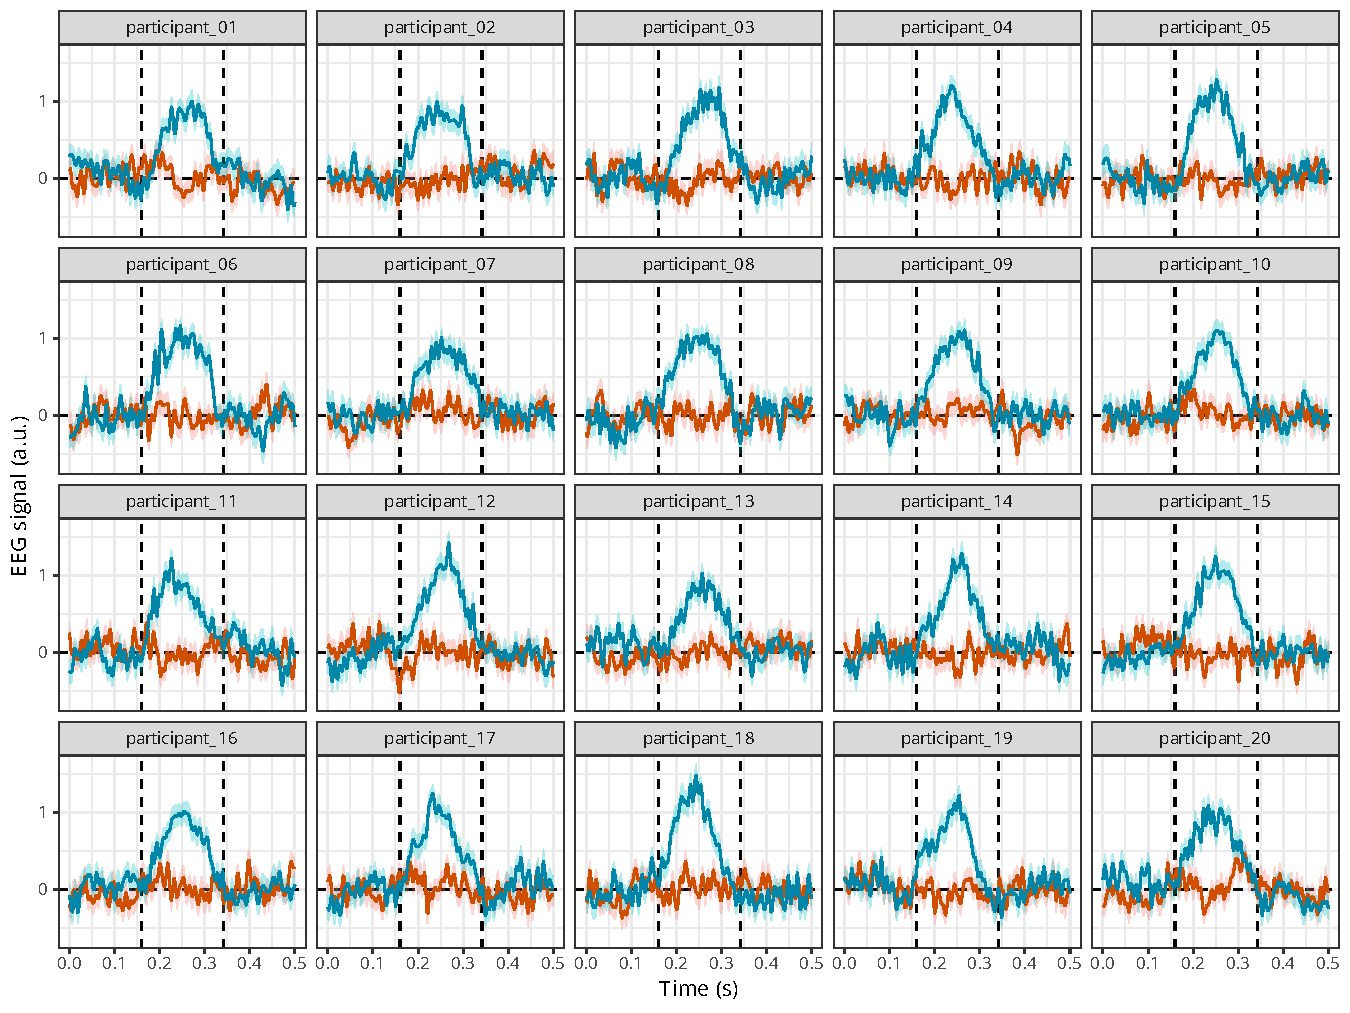
\includegraphics[width=1\textwidth,height=\textheight]{brms_meeg_files/figure-pdf/fig-eeg-1.pdf}

}

\end{figure}%

We computed the average of the ERP difference
(Figure~\ref{fig-erp})\ldots{}

\begin{figure}[!htb]

\caption{\label{fig-erp}Group-level average difference between
conditions (mean +/- standard error of the mean). The `true' onset and
offset are indicated by the vertical dashed lines.}

\centering{

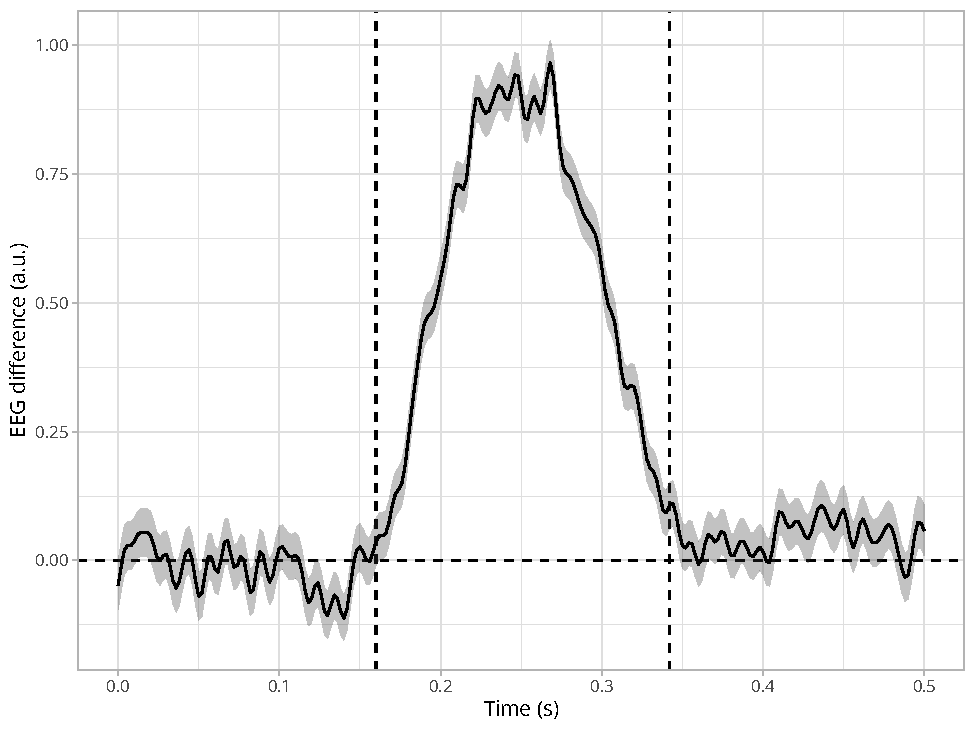
\includegraphics[width=0.75\textwidth,height=\textheight]{brms_meeg_files/figure-pdf/fig-erp-1.pdf}

}

\end{figure}%

\subsection{Model fitting}\label{model-fitting}

We then fitted a Bayesian GAM using the \texttt{brms} package
(\citeproc{ref-brms2017}{Bürkner, 2017}, \citeproc{ref-brms2018}{2018};
\citeproc{ref-nalborczyk2019}{Nalborczyk et al., 2019}). We used the
default priors in \texttt{brms} (i.e., weakly informative priors). We
ran eight Markov Chain Monte-Carlo (MCMC) to approximate the posterior
distribution, including each 5000 iterations and a warmup of 2000
iterations, yielding a total of \(8 \times (5000-2000) = 24000\)
posterior samples to use for inference. Posterior convergence was
assessed examining trace plots as well as the Gelman--Rubin statistic
\(\hat{R}\). The \texttt{brms} package uses the same syntax as the
\texttt{R} package \texttt{mgcv} v 1.9-1 (\citeproc{ref-mgcv}{Wood,
2017b}) for specifying smooth effects. Figure~\ref{fig-post-prob-test}
shows the predictions of this model together with the raw data.

\begin{Shaded}
\begin{Highlighting}[]
\CommentTok{\# averaging across participants}
\NormalTok{ppt\_df }\OtherTok{\textless{}{-}}\NormalTok{ raw\_df }\SpecialCharTok{\%\textgreater{}\%}
    \FunctionTok{group\_by}\NormalTok{(participant, condition, time) }\SpecialCharTok{\%\textgreater{}\%}
    \FunctionTok{summarise}\NormalTok{(}\AttributeTok{eeg =} \FunctionTok{mean}\NormalTok{(eeg) ) }\SpecialCharTok{\%\textgreater{}\%}
    \FunctionTok{ungroup}\NormalTok{()}

\CommentTok{\# defining a contrast for condition}
\FunctionTok{contrasts}\NormalTok{(ppt\_df}\SpecialCharTok{$}\NormalTok{condition) }\OtherTok{\textless{}{-}} \FunctionTok{c}\NormalTok{(}\SpecialCharTok{{-}}\FloatTok{0.5}\NormalTok{, }\FloatTok{0.5}\NormalTok{)}

\CommentTok{\# fitting the GAM}
\NormalTok{gam }\OtherTok{\textless{}{-}} \FunctionTok{brm}\NormalTok{(}
    \CommentTok{\# cubic regression splines with k{-}1 basis functions}
\NormalTok{    eeg }\SpecialCharTok{\textasciitilde{}}\NormalTok{ condition }\SpecialCharTok{+} \FunctionTok{s}\NormalTok{(time, }\AttributeTok{bs =} \StringTok{"cr"}\NormalTok{, }\AttributeTok{k =} \DecValTok{20}\NormalTok{, }\AttributeTok{by =}\NormalTok{ condition),}
    \AttributeTok{data =}\NormalTok{ ppt\_df,}
    \AttributeTok{family =} \FunctionTok{gaussian}\NormalTok{(),}
    \AttributeTok{warmup =} \DecValTok{2000}\NormalTok{,}
    \AttributeTok{iter =} \DecValTok{5000}\NormalTok{,}
    \AttributeTok{chains =} \DecValTok{8}\NormalTok{,}
    \AttributeTok{cores =} \DecValTok{8}\NormalTok{,}
    \AttributeTok{file =} \StringTok{"models/gam.rds"}
\NormalTok{    )}
\end{Highlighting}
\end{Shaded}

\subsection{Posterior probability of difference above
0}\label{posterior-probability-of-difference-above-0}

We then plot the posterior predictions together with the posterior
estimate of the slope for \texttt{condition} at each timestep
(Figure~\ref{fig-plot-post-slope}).

\begin{figure}[!htb]

\caption{\label{fig-plot-post-slope}Posterior estimate of the ERP in
each condition (left) or directly for the difference of ERPs (right)
according to the GAM.}

\centering{

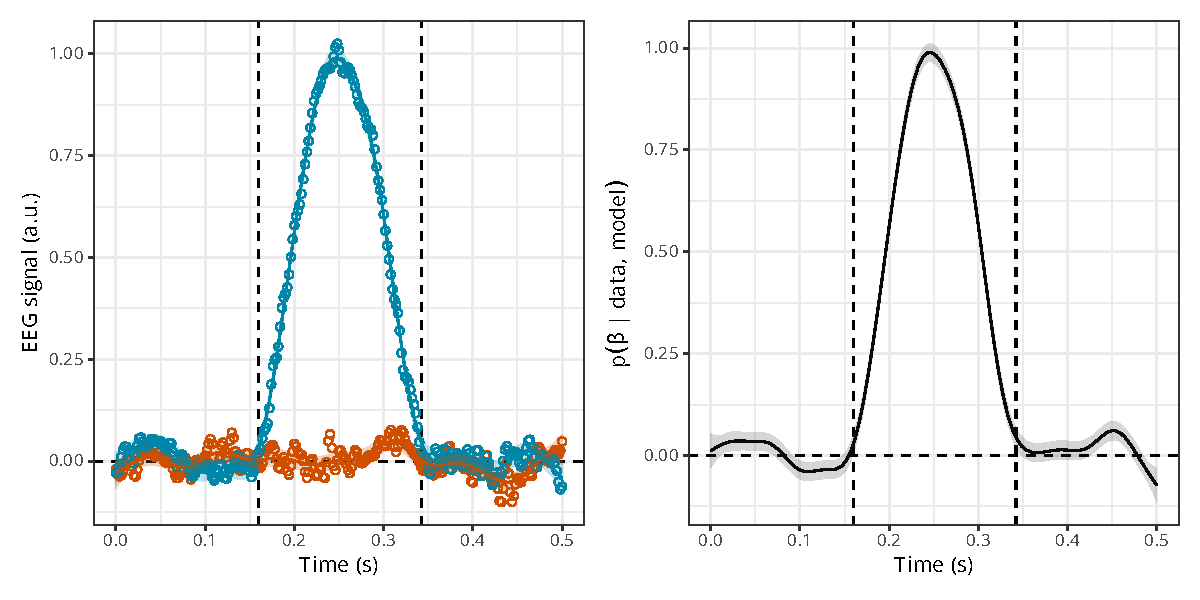
\includegraphics[width=1\textwidth,height=\textheight]{brms_meeg_files/figure-pdf/fig-plot-post-slope-1.pdf}

}

\end{figure}%

We then compute the posterior probability of the slope for
\texttt{condition} being above \(0+\epsilon\)
(Figure~\ref{fig-post-prob-test}), with \(\epsilon := 0.05\), which can
be interpreted as the smallest effect size of interest.

\begin{figure}[!htb]

\caption{\label{fig-post-prob-test}Posterior probability of the ERP
difference (slope) being above 0 according to the GAM.}

\centering{

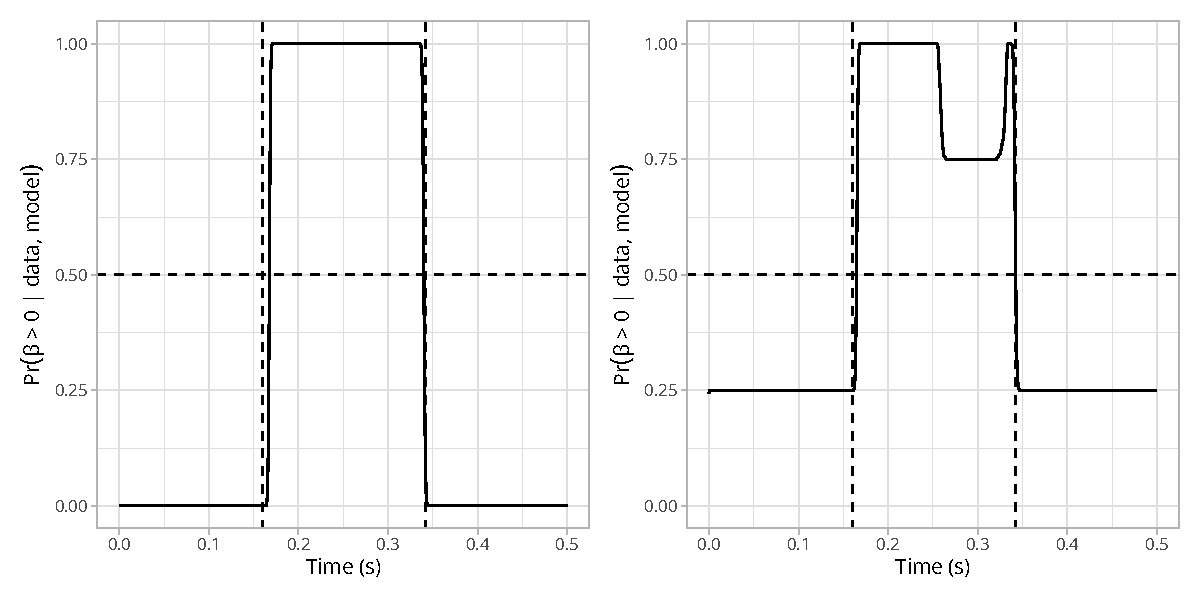
\includegraphics[width=0.75\textwidth,height=\textheight]{brms_meeg_files/figure-pdf/fig-post-prob-test-1.pdf}

}

\end{figure}%

We can also express this as the ratio of posterior probabilities (i.e.,
\(p/(1-p)\)) and visualise the timecourse of this ratio superimposed
with the conventional thresholds on evidence ratios
(Figure~\ref{fig-post-prob-ratio}).

\begin{figure}[!htb]

\caption{\label{fig-post-prob-ratio}Ratio of posterior probability
according to the GAM (on a log10 scale). Timesteps above threshold (10)
are highlighted in green.}

\centering{

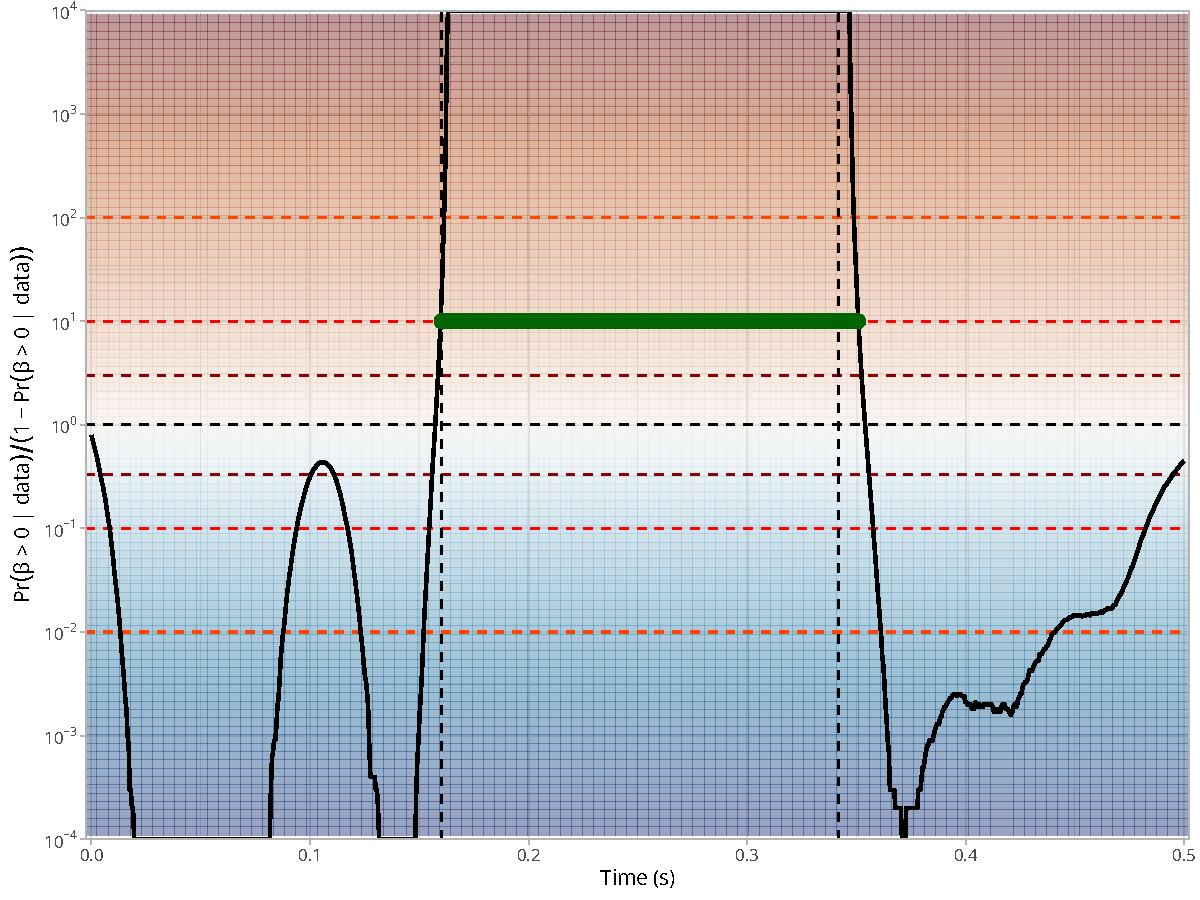
\includegraphics[width=0.75\textwidth,height=\textheight]{brms_meeg_files/figure-pdf/fig-post-prob-ratio-1.pdf}

}

\end{figure}%

\newpage

\subsection{Multilevel modelling using ERP summary
statistics}\label{multilevel-modelling-using-erp-summary-statistics}

Next we fit a hierarchical/multilevel GAM using summary statistics of
ERPs (mean and SD) at the participant level (similar to what is done in
meta-analysis). Although it is possible to fit a GAMM at the
single-trial level, we present a resource-efficient version of the model
that is fitted directly on the by-participant summary statistics (mean
and SD)\ldots{}

\begin{Shaded}
\begin{Highlighting}[]
\CommentTok{\# averaging across participants}
\NormalTok{summary\_df }\OtherTok{\textless{}{-}}\NormalTok{ raw\_df }\SpecialCharTok{\%\textgreater{}\%}
    \FunctionTok{summarise}\NormalTok{(}
        \AttributeTok{eeg\_mean =} \FunctionTok{mean}\NormalTok{(eeg),}
        \AttributeTok{eeg\_sd =} \FunctionTok{sd}\NormalTok{(eeg),}
        \AttributeTok{.by =} \FunctionTok{c}\NormalTok{(participant, condition, time)}
\NormalTok{        )}

\CommentTok{\# defining a contrast for condition}
\FunctionTok{contrasts}\NormalTok{(summary\_df}\SpecialCharTok{$}\NormalTok{condition) }\OtherTok{\textless{}{-}} \FunctionTok{c}\NormalTok{(}\SpecialCharTok{{-}}\FloatTok{0.5}\NormalTok{, }\FloatTok{0.5}\NormalTok{)}

\CommentTok{\# fitting the GAM}
\NormalTok{meta\_gam }\OtherTok{\textless{}{-}} \FunctionTok{brm}\NormalTok{(}
    \CommentTok{\# using by{-}participant SD of ERPs across trials}
\NormalTok{    eeg\_mean }\SpecialCharTok{|} \FunctionTok{se}\NormalTok{(eeg\_sd) }\SpecialCharTok{\textasciitilde{}}
\NormalTok{        condition }\SpecialCharTok{+} \FunctionTok{s}\NormalTok{(time, }\AttributeTok{bs =} \StringTok{"cr"}\NormalTok{, }\AttributeTok{k =} \DecValTok{20}\NormalTok{, }\AttributeTok{by =}\NormalTok{ condition) }\SpecialCharTok{+}
\NormalTok{        (}\DecValTok{1} \SpecialCharTok{|}\NormalTok{ participant),}
    \AttributeTok{data =}\NormalTok{ summary\_df,}
    \AttributeTok{family =} \FunctionTok{gaussian}\NormalTok{(),}
    \AttributeTok{warmup =} \DecValTok{2000}\NormalTok{,}
    \AttributeTok{iter =} \DecValTok{5000}\NormalTok{,}
    \AttributeTok{chains =} \DecValTok{8}\NormalTok{,}
    \AttributeTok{cores =} \DecValTok{8}\NormalTok{,}
    \AttributeTok{file =} \StringTok{"models/meta\_gam.rds"}
\NormalTok{    )}
\end{Highlighting}
\end{Shaded}

\subsection{Error properties of the proposed
approach}\label{error-properties-of-the-proposed-approach}

We then computed the difference between the true and estimated
onset/offset of the ERP difference
(\(\text{error}:=|\hat{\theta}-\theta|\)), according to various
\texttt{eps} and \texttt{threshold} values. Remember that the signal is
generated from a truncated Gaussian with an objective onset at 160 ms, a
maximum at 250 ms, and an offset at 342 ms. Figure~\ref{fig-onset-error}
shows that the hierarchical GAM can \emph{exactly} recover the true
onset and offset values, given some reasonable choice of \texttt{eps}
and \texttt{threshold} values (e.g., a threshold of 20).

\begin{verbatim}
   eps threshold estimated_onset estimated_offset error_onset error_offset
1 0.00        13            0.16             0.34           0        0.002
2 0.00        14            0.16             0.34           0        0.002
3 0.00        15            0.16             0.34           0        0.002
4 0.00        16            0.16             0.34           0        0.002
5 0.00        17            0.16             0.34           0        0.002
6 0.01        10            0.16             0.34           0        0.002
\end{verbatim}

\begin{figure}[!htb]

\caption{\label{fig-onset-error}Error function of onset (left) and
offset (right) estimation according to various eps and threshold values
(according to the hierarchical GAM). Minimum error values are indicated
by red crosses.}

\centering{

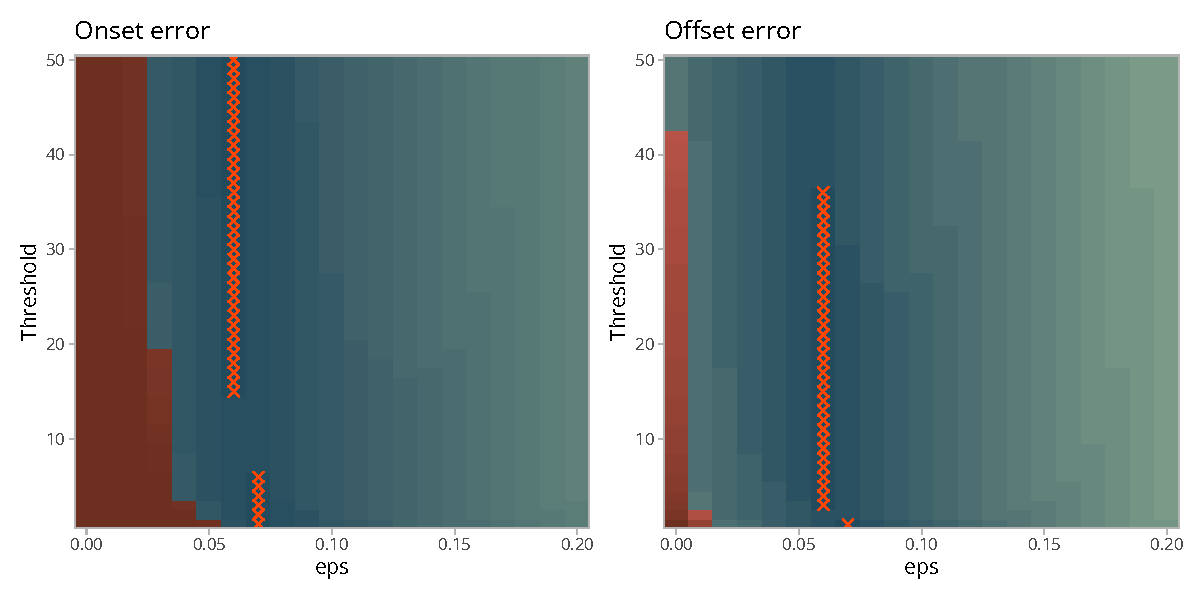
\includegraphics[width=1\textwidth,height=\textheight]{brms_meeg_files/figure-pdf/fig-onset-error-1.pdf}

}

\end{figure}%

\newpage

\subsection{Comparing the identified onsets/offsets to other
approaches}\label{comparing-the-identified-onsetsoffsets-to-other-approaches}

We compared the ability of the GAMM to correctly estimate the onset and
offset of the ERP difference to widely used methods. First, we conducted
mass-univariate t-tests (thus treating each timestep independently) and
identified the onset and offset of the ERP difference as the first and
last values crossing an arbitrary significance threshold
(\(\alpha = 0.01\)). We then followed the same approach but after
applying different forms of multiplicity correction the the p-values. We
compared two methods that control the false discovery rate (FDR) (i.e.,
BH95, \citeproc{ref-benjamini1995}{Benjamini \& Hochberg, 1995}; and
BY01, \citeproc{ref-benjamini2001}{Benjamini \& Yekutieli, 2001}), one
method that controls the familywise error rate (FWER) (i.e.,
Holm--Bonferroni method, \citeproc{ref-holm1979}{Holm, 1979}), and two
cluster-based methods (permutation with a single threshold and TFCE,
\citeproc{ref-smith2009}{S. Smith \& Nichols, 2009}). The BH95, BY01,
and Holm corrections were applied to the p-values using the
\texttt{p.adjust()} function in \texttt{R}. The cluster-based inference
was implemented using a cluster-sum statistic of squared t-values, as
implemented in \texttt{MNE-Python}
(\citeproc{ref-gramfort2013}{Gramfort, 2013}), called via the \texttt{R}
package \texttt{reticulate} v 1.35.0 (\citeproc{ref-reticulate}{Ushey et
al., 2024}). We also compared these estimates to the onset and offset as
estimated using the binary segmentation algorithm, as implemented in the
\texttt{R} package \texttt{changepoint} v 2.2.4
(\citeproc{ref-changepoint}{Killick et al., 2022a}), and applied
directly to the squared t-values (as in
\citeproc{ref-rousselet_using_2025}{Rousselet, 2025}). For visualisation
and interpretability purposes, we converted p-values to s-values, which
can be interpreted as bits of surprising information, assuming a null
effect (\citeproc{ref-greenland2019}{Greenland, 2019})
(Figure~\ref{fig-corrections}).

\begin{figure}[!htb]

\caption{\label{fig-corrections}Timecourse of squared t-values and
s-values, with true onset (black dashed line) and onsets identified
using the raw (uncorrected) p-values or the corrected p-values (BH, BY,
Holm).}

\centering{

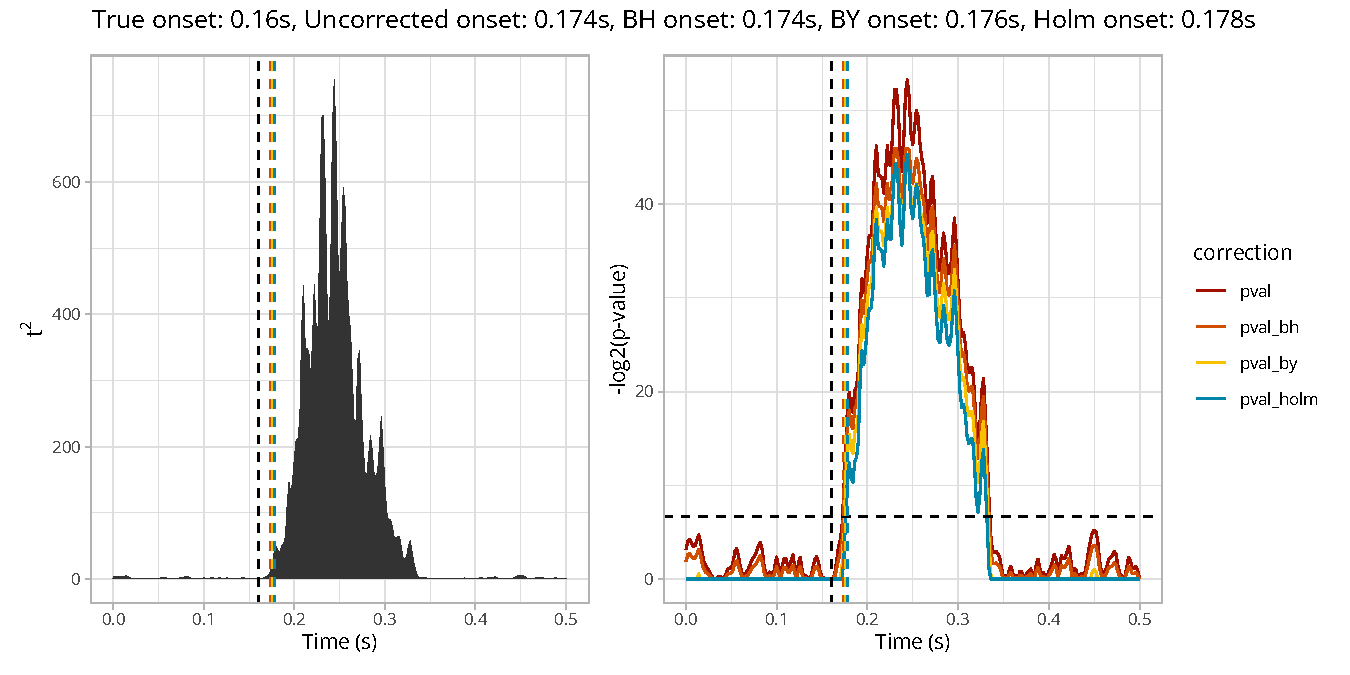
\includegraphics[width=1\textwidth,height=\textheight]{brms_meeg_files/figure-pdf/fig-corrections-1.pdf}

}

\end{figure}%

\newpage

\subsection{Simulation study}\label{simulation-study}

Onset/offset estimation methods were assessed using the median absolute
error (MAE) and variance of 10.000 simulated datasets\ldots{}

\subsection{Application to actual MEG
data}\label{application-to-actual-meg-data}

Next, we assessed the performance of the proposed approach on actual MEG
data (decoding results of Nalborczyk et al., in preparation). We
conducted time-resolved multivariate pattern analysis (MVPA), also known
as decoding\ldots{} As a result, we have a timecourse of decoding
performance (ROC AUC), bounded between 0 and 1, for each participant
(for a total of 32 participants). Now, we want to \emph{test} whether
the group-level average decoding accuracy is above chance (i.e., 0.5) at
each timestep (Figure~\ref{fig-decoding-data}). We fitted a similar GAM
as discussed previously, but we replaced the \(\mathrm{Normal}\)
likelihood function by a \(\mathrm{Beta}\) one to account for the
bounded nature of AUC values (between 0 and 1) (for a tutorial on Beta
regression, see \citeproc{ref-coretta2025}{Coretta \& Bürkner, 2025}).
Note that although we chose a basis dimension of \(k=50\), which seems
appropriate for the present data, this choice should be adapted
according to the properties of the modelled data (e.g., signal-to-noise
ratio, prior low-pass filtering, sampling rate, etc) and should be
assessed by the usual model checking tools (e.g., posterior predictive
checks). We also define a region of practical equivalence (ROPE,
\citeproc{ref-kruschke2017}{Kruschke \& Liddell, 2017}), defined as the
chance level plus the standard deviation of the (group-level average)
decoding performance during the baseline period. This ensures
that\ldots{}\footnote{Could an alternative approach be to include a
  predictor for ``baseline vs.~after baseline''?}

\begin{Shaded}
\begin{Highlighting}[]
\CommentTok{\# fitting the Beta GAM}
\NormalTok{meg\_decoding\_gam }\OtherTok{\textless{}{-}} \FunctionTok{brm}\NormalTok{(}
\NormalTok{    auc }\SpecialCharTok{\textasciitilde{}} \FunctionTok{s}\NormalTok{(time, }\AttributeTok{bs =} \StringTok{"cr"}\NormalTok{, }\AttributeTok{k =} \DecValTok{50}\NormalTok{),}
    \AttributeTok{data =}\NormalTok{ decoding\_df,}
    \AttributeTok{family =} \FunctionTok{Beta}\NormalTok{(),}
    \AttributeTok{warmup =} \DecValTok{2000}\NormalTok{,}
    \AttributeTok{iter =} \DecValTok{5000}\NormalTok{,}
    \AttributeTok{chains =} \DecValTok{4}\NormalTok{,}
    \AttributeTok{cores =} \DecValTok{4}
\NormalTok{    )}
\end{Highlighting}
\end{Shaded}

We assessed the reliability of the proposed approach using a form of
permutation-based split-half reliability (e.g.,
\citeproc{ref-rosenblatt2018}{Rosenblatt et al., 2018}), which consisted
of the following steps:

\begin{itemize}
\tightlist
\item
  Create many (e.g., 10 or 20) half train/test splits of the data
\item
  For each fold, estimate the onset/offset on both splits using all
  methods
\item
  Then summarise the distribution of onset/offset with the median and
  variance across folds
\end{itemize}

This will allow checking that the proposed approach produces reliable
onset/offset estimates.

\begin{figure}[!htb]

\caption{\label{fig-decoding-data}Group-level average decoding
performance (N=32) superimposed with the GAM predictions (in blue) and
the region of practical equivalence (ROPE, in orange) computed from the
baseline period. The blue horizontal line indicates the timesteps at
which the posterior probability ratio is equal to or greater than 20.}

\centering{

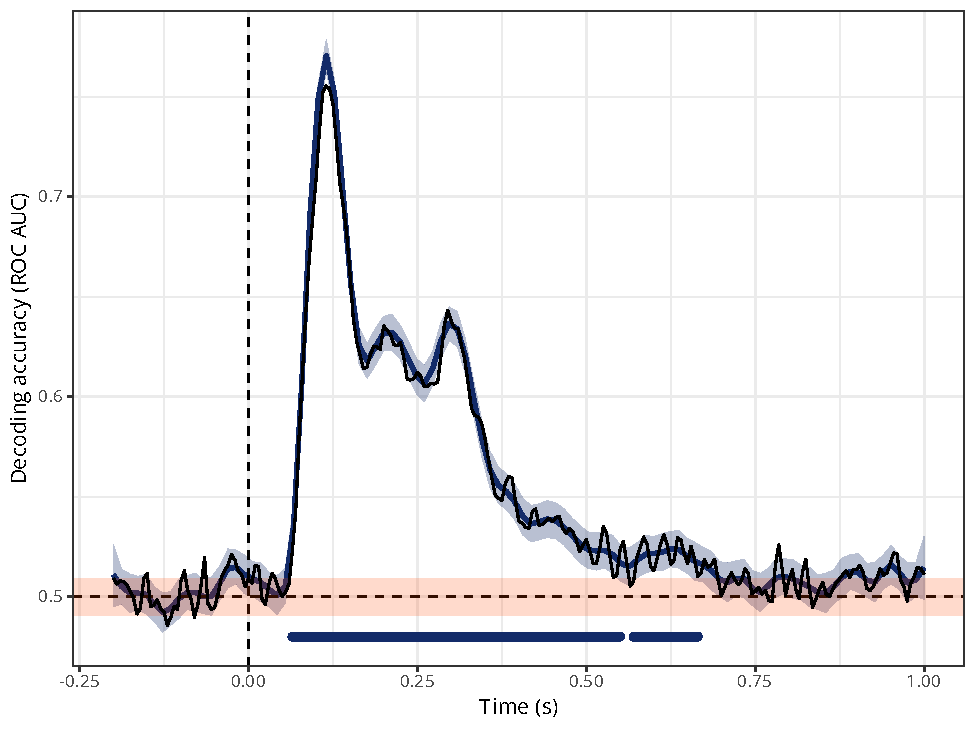
\includegraphics[width=0.75\textwidth,height=\textheight]{brms_meeg_files/figure-pdf/fig-decoding-data-1.pdf}

}

\end{figure}%

\newpage

\section{Results}\label{results}

This section is divided in two parts. First, we present the results from
the simulation study, assessing the bias and variance of each method
when applied to simulated data in which the ground truth is known.
Second, we present the results obtained when applying the different
methods to actual MEG data (decoding performance through time),
assessing the reliability of each method and the stability of its
estimates.

\subsection{Simulation results (bias and
variance)}\label{simulation-results-bias-and-variance}

Figure~\ref{fig-simulation-mae-variance} shows a summary of the
simulation results, revealing that the proposed approach (\texttt{brms})
has the lowest MAE and variance for both the onset and offset
estimates\ldots{}

\begin{figure}[!htb]

\caption{\label{fig-simulation-mae-variance}Median absolute error and
variance of onset and offset estimates for each method.}

\centering{

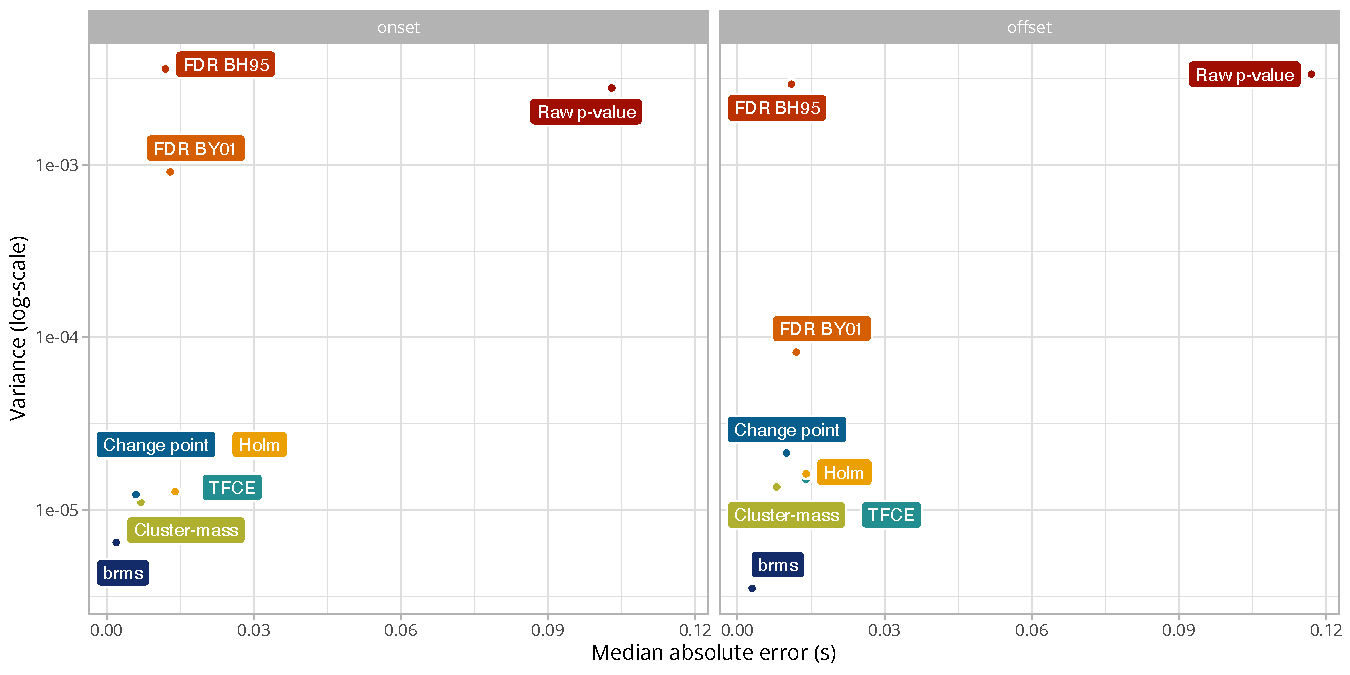
\includegraphics[width=1\textwidth,height=\textheight]{brms_meeg_files/figure-pdf/fig-simulation-mae-variance-1.pdf}

}

\end{figure}%

\begin{figure}[!htb]

\caption{\label{fig-simulation-distribution}Distributions of onset and
offset estimates for each method.}

\centering{

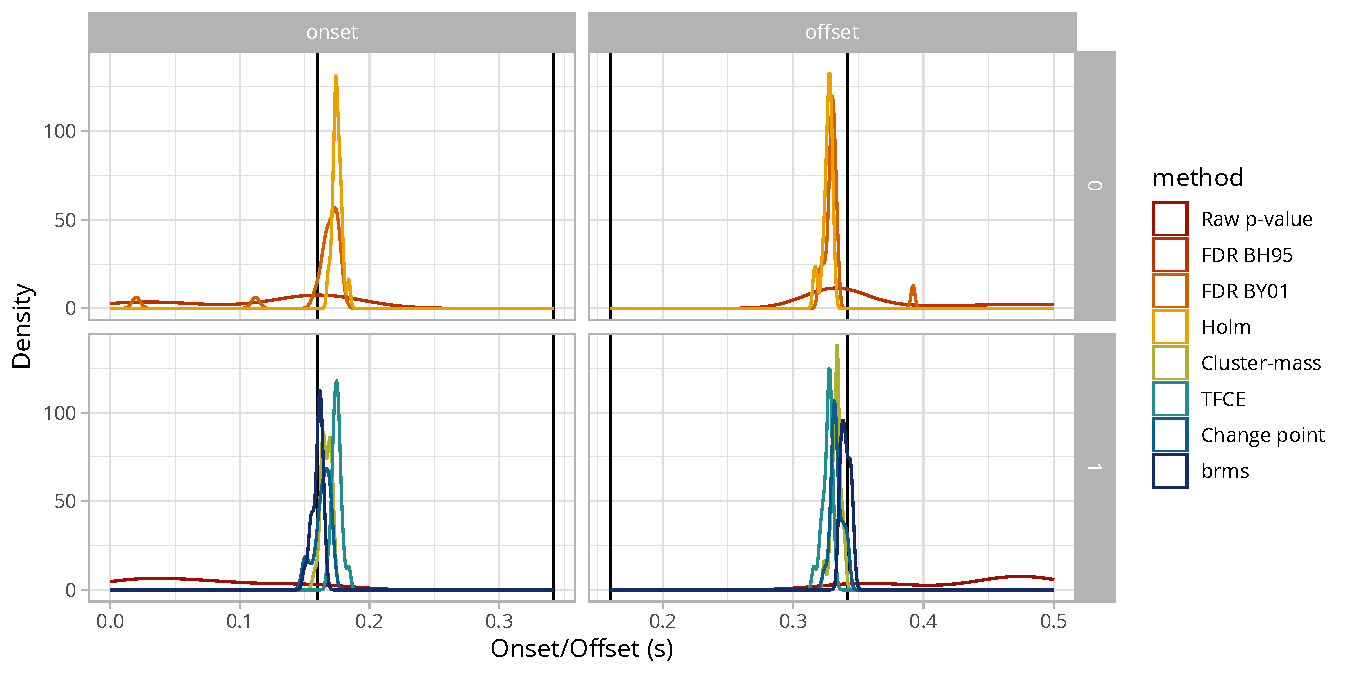
\includegraphics[width=1\textwidth,height=\textheight]{brms_meeg_files/figure-pdf/fig-simulation-distribution-1.pdf}

}

\end{figure}%

\newpage

\subsection{Application to actual MEG data
(reliability)}\label{application-to-actual-meg-data-reliability}

Figure~\ref{fig-onset-offset} shows the group-level average decoding
performance through time with onset and offset estimates for each
method. The \texttt{brms\_full} method is similar to the \texttt{brms}
method except that the ROPE is defined on the entire dataset rather than
on the split dataset. Overall, this figure shows that both the
\texttt{Raw\ p-value} and \texttt{FDR\ BH95} methods were extremely
lenient, considering that the decoding performance was above chance
before the onset of the stimulus (false positive) and until the end of
the trial. The \texttt{Change\ point} and \texttt{Cluster\ mass} methods
were the most conservative methods, identifying a time window from
approximately +60ms to +500ms. The \texttt{Holm}, \texttt{TFCE},
\texttt{brms}, and \texttt{brms\_full} methods produced somewhat similar
estimates of onset and offset, from approximately +60ms to
+650ms.\footnote{It should be noted that although each method can
  produce several ``clusters'' of timesteps, we only considered the
  first (onset) and last (offset) timesteps identified by each method to
  compute the error (difference).}

\begin{figure}[!htb]

\caption{\label{fig-onset-offset}Group-level average decoding
performance through time with onset and offset estimates for each method
(data from Nalborczyk et al., in preparation).}

\centering{

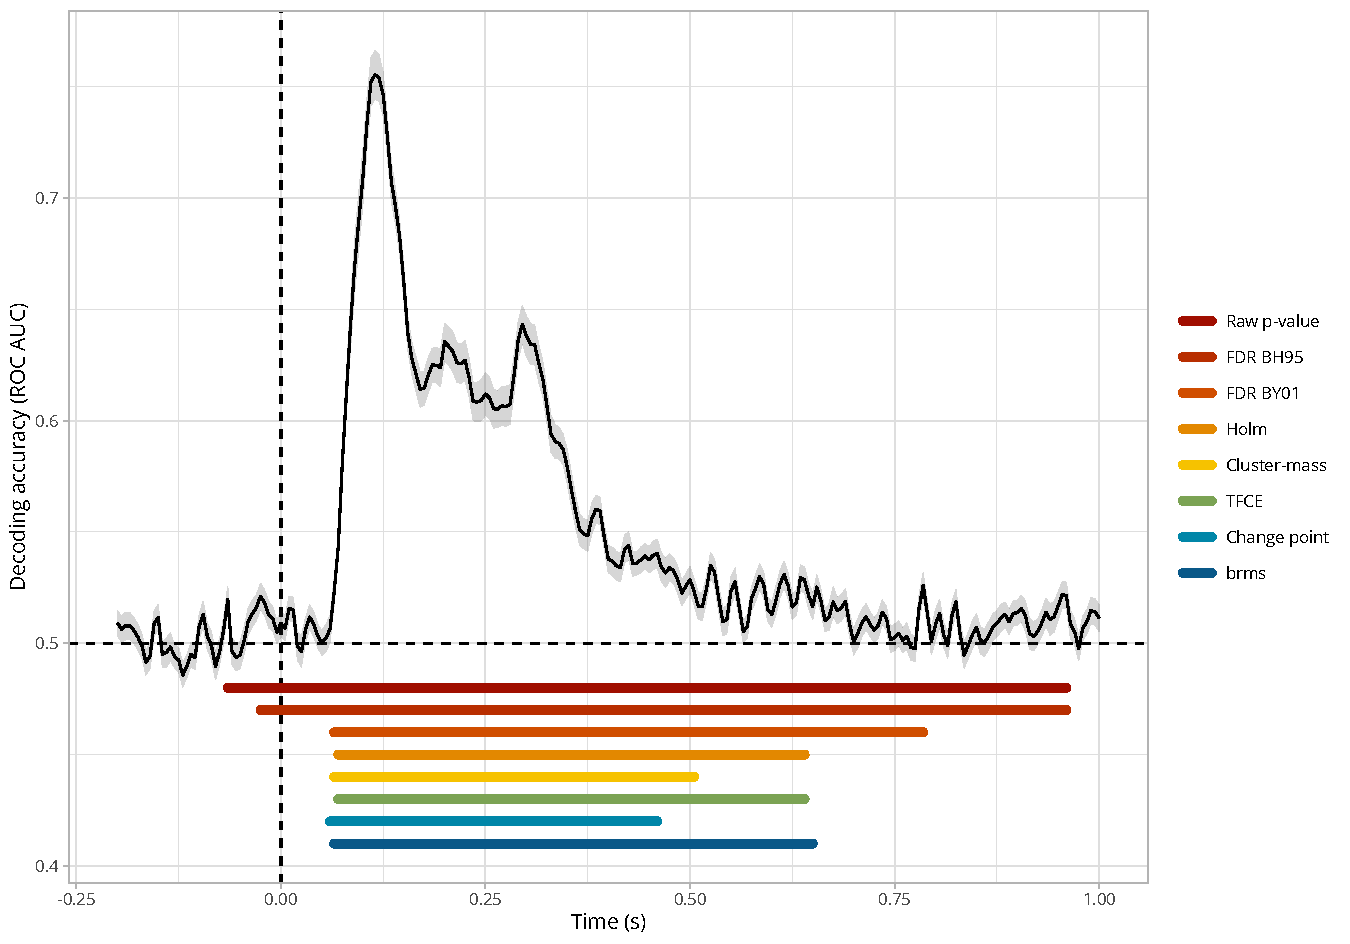
\includegraphics[width=1\textwidth,height=\textheight]{brms_meeg_files/figure-pdf/fig-onset-offset-1.pdf}

}

\end{figure}%

Figure~\ref{fig-reliability} shows two properties of each method: i) the
median difference between the onset and offset estimates from each data
split and the onset and offset estimates from the full dataset (x-axis)
and ii) and the variance of its onset and offset estimates across data
splits (y-axis). This figure reveals that the \texttt{brms} \emph{onset
and offset} estimates on each split are the closest to the estimates
from the full dataset on average (0ms difference for the onset estimate
and 5ms difference for the offset estimate). The \texttt{Raw\ p-value}
method has similar performance, but given the aberrant estimates it
produces (cf. Figure~\ref{fig-onset-offset}), the result that it is
consistent between data splits and the full dataset is not convincing on
its own. Overall, the figure reveals that for all other methods, split
datasets produce later onset estimates and earlier offset estimates (as
compared to the estimates from the model fitted on the full dataset).

\begin{figure}[!htb]

\caption{\label{fig-reliability}Median absolute error and variance of
onset (left) and offset (right) estimates for each method.}

\centering{

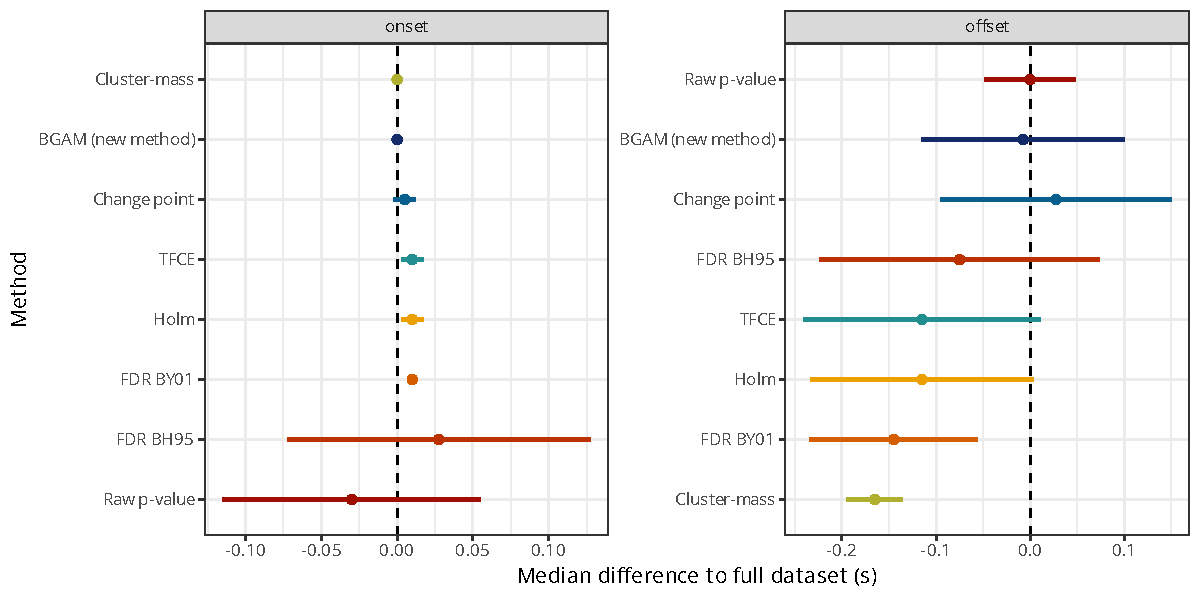
\includegraphics[width=1\textwidth,height=\textheight]{brms_meeg_files/figure-pdf/fig-reliability-1.pdf}

}

\end{figure}%

\newpage

\section{Discussion}\label{discussion}

\ldots{}

\subsection{Summary of the proposed
approach}\label{summary-of-the-proposed-approach}

Overall, before concluding on the onset/offset of effect based on the
model, we need to ensure that the model provides a faithful description
of the data-generating process (e.g., via posterior predictive checks
etc)\ldots{}

\subsection{Increasing potential
usage}\label{increasing-potential-usage}

Prepare a wrapper \texttt{R} package and show how to call it in
\texttt{Python} and integrate it with \texttt{MNE-Python}
(\citeproc{ref-gramfort2013}{Gramfort, 2013}) pipelines\ldots{}

\subsection{Limitations and future
directions}\label{limitations-and-future-directions}

As in previous simulation work (e.g.,
\citeproc{ref-rousselet2008}{Rousselet et al., 2008};
\citeproc{ref-sassenhagen2019}{Sassenhagen \& Draschkow, 2019}), the
present simulation results depend on various choices such as the
specific cluster-forming algorithm and threshold, signal-to-noise ratio,
negative impact of preprocessing steps (e.g., low-pass filter) on
temporal resolution\ldots{} note however, that the same caveats apply to
all methods\ldots{}

The error properties depend on the threshold parameter, a value of 10 or
20 seems to be a reasonable default, but the optimal threshold parameter
can be adjusted using split-half reliability assessment\ldots{}

Can be applied to any 1D timeseries (e.g., pupillometry,
electromyography)\ldots{} Extending the approach to spatiotemporal data
(i.e., time + sensors)\ldots{}

We kept the exemplary models simple, but can be extended by adding
varying/random effects (intercept and slope) for item (e.g.,
word)\ldots{} but also continuous predictors at the trial level?

\subsection{Conclusions}\label{conclusions}

\ldots{}

\newpage

\section{Data and code availability}\label{data-and-code-availability}

The simulation results as well as the \texttt{R} code to reproduce the
simulations are available on GitHub:
\url{https://github.com/lnalborczyk/brms_meeg}.

\section{Packages}\label{packages}

We used R version 4.2.3 (\citeproc{ref-base}{R Core Team, 2023}) and the
following R packages: brms v. 2.22.0 (\citeproc{ref-brms2017}{Bürkner,
2017}, \citeproc{ref-brms2018}{2018}, \citeproc{ref-brms2021}{2021}),
changepoint v. 2.2.4 (\citeproc{ref-changepoint2022}{Killick et al.,
2022b}; \citeproc{ref-changepoint2014}{Killick \& Eckley, 2014}),
grateful v. 0.2.10 (\citeproc{ref-grateful}{Rodriguez-Sanchez \&
Jackson, 2023}), knitr v. 1.45 (\citeproc{ref-knitr2014}{Xie, 2014},
\citeproc{ref-knitr2015}{2015}, \citeproc{ref-knitr2023}{2023}),
MetBrewer v. 0.2.0 (\citeproc{ref-MetBrewer}{Mills, 2022}), pakret v.
0.2.2 (\citeproc{ref-pakret}{Gallou, 2024}), patchwork v. 1.2.0
(\citeproc{ref-patchwork}{T. L. Pedersen, 2024}), rmarkdown v. 2.29
(\citeproc{ref-rmarkdown2024}{Allaire et al., 2024};
\citeproc{ref-rmarkdown2018}{Xie et al., 2018},
\citeproc{ref-rmarkdown2020}{2020}), scales v. 1.3.0
(\citeproc{ref-scales}{Wickham et al., 2023}), scico v. 1.5.0
(\citeproc{ref-scico}{T. L. Pedersen \& Crameri, 2023}), tidybayes v.
3.0.6 (\citeproc{ref-tidybayes}{Kay, 2023}), tidyverse v. 2.0.0
(\citeproc{ref-tidyverse}{Wickham et al., 2019}).

\newpage

\section{References}\label{references}

\phantomsection\label{refs}
\begin{CSLReferences}{1}{0}
\bibitem[\citeproctext]{ref-abugaber2023}
Abugaber, D., Finestrat, I., Luque, A., \& Morgan-Short, K. (2023).
Generalized additive mixed modeling of EEG supports dual-route accounts
of morphosyntax in suggesting no word frequency effects on processing of
regular grammatical forms. \emph{Journal of Neurolinguistics},
\emph{67}, 101137.
\url{https://doi.org/10.1016/j.jneuroling.2023.101137}

\bibitem[\citeproctext]{ref-rmarkdown2024}
Allaire, J., Xie, Y., Dervieux, C., McPherson, J., Luraschi, J., Ushey,
K., Atkins, A., Wickham, H., Cheng, J., Chang, W., \& Iannone, R.
(2024). \emph{{rmarkdown}: Dynamic documents for r}.
\url{https://github.com/rstudio/rmarkdown}

\bibitem[\citeproctext]{ref-baayen2020}
Baayen, R. H., \& Linke, M. (2020). \emph{Generalized Additive Mixed
Models} (pp. 563--591). Springer International Publishing.
\url{https://doi.org/10.1007/978-3-030-46216-1_23}

\bibitem[\citeproctext]{ref-baayen2018}
Baayen, R. H., Rij, J. van, Cat, C. de, \& Wood, S. (2018).
\emph{Autocorrelated errors in experimental data in the language
sciences: Some solutions offered by generalized additive mixed models}
(pp. 49--69). Springer International Publishing.
\url{https://doi.org/10.1007/978-3-319-69830-4_4}

\bibitem[\citeproctext]{ref-benjamini1995}
Benjamini, Y., \& Hochberg, Y. (1995). Controlling the False Discovery
Rate: A Practical and Powerful Approach to Multiple Testing.
\emph{Journal of the Royal Statistical Society Series B: Statistical
Methodology}, \emph{57}(1), 289--300.
\url{https://doi.org/10.1111/j.2517-6161.1995.tb02031.x}

\bibitem[\citeproctext]{ref-benjamini2001}
Benjamini, Y., \& Yekutieli, D. (2001). The control of the false
discovery rate in multiple testing under dependency. \emph{The Annals of
Statistics}, \emph{29}(4). \url{https://doi.org/10.1214/aos/1013699998}

\bibitem[\citeproctext]{ref-brms2017}
Bürkner, P.-C. (2017). {brms}: An {R} package for {Bayesian} multilevel
models using {Stan}. \emph{Journal of Statistical Software},
\emph{80}(1), 1--28. \url{https://doi.org/10.18637/jss.v080.i01}

\bibitem[\citeproctext]{ref-brms2018}
Bürkner, P.-C. (2018). Advanced {Bayesian} multilevel modeling with the
{R} package {brms}. \emph{The R Journal}, \emph{10}(1), 395--411.
\url{https://doi.org/10.32614/RJ-2018-017}

\bibitem[\citeproctext]{ref-brms2021}
Bürkner, P.-C. (2021). Bayesian item response modeling in {R} with
{brms} and {Stan}. \emph{Journal of Statistical Software},
\emph{100}(5), 1--54. \url{https://doi.org/10.18637/jss.v100.i05}

\bibitem[\citeproctext]{ref-combrisson_exceeding_2015}
Combrisson, E., \& Jerbi, K. (2015). Exceeding chance level by chance:
{The} caveat of theoretical chance levels in brain signal classification
and statistical assessment of decoding accuracy. \emph{Journal of
Neuroscience Methods}, \emph{250}, 126--136.
\url{https://doi.org/10.1016/j.jneumeth.2015.01.010}

\bibitem[\citeproctext]{ref-coretta2025}
Coretta, S., \& Bürkner, P.-. C. (2025). \emph{Bayesian beta regressions
with brms in r: A tutorial for phoneticians}.
\url{http://dx.doi.org/10.31219/osf.io/f9rqg_v1}

\bibitem[\citeproctext]{ref-dimigen2021}
Dimigen, O., \& Ehinger, B. V. (2021). Regression-based analysis of
combined EEG and eye-tracking data: Theory and applications.
\emph{Journal of Vision}, \emph{21}(1), 3.
\url{https://doi.org/10.1167/jov.21.1.3}

\bibitem[\citeproctext]{ref-dinga2021}
Dinga, R., Fraza, C. J., Bayer, J. M. M., Kia, S. M., Beckmann, C. F.,
\& Marquand, A. F. (2021). \emph{Normative modeling of neuroimaging data
using generalized additive models of location scale and shape}.
\url{http://dx.doi.org/10.1101/2021.06.14.448106}

\bibitem[\citeproctext]{ref-dunagan2024}
Dunagan, D., Jordan, T., Hale, J. T., Pylkkänen, L., \& Chacón, D. A.
(2024). \emph{Evaluating the timecourses of morpho-orthographic,
lexical, and grammatical processing following rapid parallel visual
presentation: An EEG investigation in english}.
\url{http://dx.doi.org/10.1101/2024.04.10.588861}

\bibitem[\citeproctext]{ref-ehinger_unfold_2019}
Ehinger, B. V., \& Dimigen, O. (2019). Unfold: An integrated toolbox for
overlap correction, non-linear modeling, and regression-based {EEG}
analysis. \emph{PeerJ}, \emph{7}, e7838.
\url{https://doi.org/10.7717/peerj.7838}

\bibitem[\citeproctext]{ref-eklund2016}
Eklund, A., Nichols, T. E., \& Knutsson, H. (2016). Cluster failure: Why
fMRI inferences for spatial extent have inflated false-positive rates.
\emph{Proceedings of the National Academy of Sciences}, \emph{113}(28),
7900--7905. \url{https://doi.org/10.1073/pnas.1602413113}

\bibitem[\citeproctext]{ref-fischer2013}
Fischer, Adrian~G., \& Ullsperger, M. (2013). Real and Fictive Outcomes
Are Processed Differently but Converge on a Common Adaptive Mechanism.
\emph{Neuron}, \emph{79}(6), 1243--1255.
\url{https://doi.org/10.1016/j.neuron.2013.07.006}

\bibitem[\citeproctext]{ref-frossard2021}
Frossard, J., \& Renaud, O. (2021). Permutation Tests for Regression,
ANOVA, and Comparison of Signals: The {\textbf{permuco}} Package.
\emph{Journal of Statistical Software}, \emph{99}(15).
\url{https://doi.org/10.18637/jss.v099.i15}

\bibitem[\citeproctext]{ref-frossard2022}
Frossard, J., \& Renaud, O. (2022). The cluster depth tests: Toward
point-wise strong control of the family-wise error rate in massively
univariate tests with application to M/EEG. \emph{NeuroImage},
\emph{247}, 118824.
\url{https://doi.org/10.1016/j.neuroimage.2021.118824}

\bibitem[\citeproctext]{ref-pakret}
Gallou, A. (2024). \emph{{pakret}: Cite {``{R}''} packages on the fly in
{``{R Markdown}''} and {``{Quarto}''}}.
\url{https://CRAN.R-project.org/package=pakret}

\bibitem[\citeproctext]{ref-gramfort2013}
Gramfort, A. (2013). MEG and EEG data analysis with MNE-python.
\emph{Frontiers in Neuroscience}, \emph{7}.
\url{https://doi.org/10.3389/fnins.2013.00267}

\bibitem[\citeproctext]{ref-greenland2019}
Greenland, S. (2019). Valid {\emph{P}} -Values Behave Exactly as They
Should: Some Misleading Criticisms of {\emph{P}} -Values and Their
Resolution With {\emph{S}} -Values. \emph{The American Statistician},
\emph{73}(sup1), 106--114.
\url{https://doi.org/10.1080/00031305.2018.1529625}

\bibitem[\citeproctext]{ref-hastie2017}
Hastie, T. J., \& Tibshirani, R. J. (2017). \emph{Generalized Additive
Models}. Routledge. \url{https://doi.org/10.1201/9780203753781}

\bibitem[\citeproctext]{ref-hauk2006}
Hauk, O., Davis, M. H., Ford, M., Pulvermüller, F., \& Marslen-Wilson,
W. D. (2006). The time course of visual word recognition as revealed by
linear regression analysis of ERP data. \emph{NeuroImage}, \emph{30}(4),
1383--1400. \url{https://doi.org/10.1016/j.neuroimage.2005.11.048}

\bibitem[\citeproctext]{ref-hayasaka_validating_2003}
Hayasaka, S. (2003). Validating cluster size inference: Random field and
permutation methods. \emph{NeuroImage}, \emph{20}(4), 2343--2356.
\url{https://doi.org/10.1016/j.neuroimage.2003.08.003}

\bibitem[\citeproctext]{ref-hendrix2017}
Hendrix, P., Bolger, P., \& Baayen, H. (2017). Distinct ERP signatures
of word frequency, phrase frequency, and prototypicality in speech
production. \emph{Journal of Experimental Psychology: Learning, Memory,
and Cognition}, \emph{43}(1), 128--149.
\url{https://doi.org/10.1037/a0040332}

\bibitem[\citeproctext]{ref-holm1979}
Holm, S. (1979). A simple sequentially rejective multiple test
procedure. \emph{Scandinavian Journal of Statistics}, \emph{6}(2),
65--70. \url{http://www.jstor.org/stable/4615733}

\bibitem[\citeproctext]{ref-tidybayes}
Kay, M. (2023). \emph{{tidybayes}: Tidy data and geoms for {Bayesian}
models}. \url{https://doi.org/10.5281/zenodo.1308151}

\bibitem[\citeproctext]{ref-changepoint2014}
Killick, R., \& Eckley, I. A. (2014). {changepoint}: An {R} package for
changepoint analysis. \emph{Journal of Statistical Software},
\emph{58}(3), 1--19.
\url{https://www.jstatsoft.org/article/view/v058i03}

\bibitem[\citeproctext]{ref-changepoint}
Killick, R., Haynes, K., \& Eckley, I. A. (2022a). \emph{{changepoint}:
An {R} package for changepoint analysis}.
\url{https://CRAN.R-project.org/package=changepoint}

\bibitem[\citeproctext]{ref-changepoint2022}
Killick, R., Haynes, K., \& Eckley, I. A. (2022b). \emph{{changepoint}:
An {R} package for changepoint analysis}.
\url{https://CRAN.R-project.org/package=changepoint}

\bibitem[\citeproctext]{ref-king2014}
King, J.-R., \& Dehaene, S. (2014). Characterizing the dynamics of
mental representations: the temporal generalization method. \emph{Trends
in Cognitive Sciences}, \emph{18}(4), 203--210.
\url{https://doi.org/10.1016/j.tics.2014.01.002}

\bibitem[\citeproctext]{ref-kruschke2017}
Kruschke, J. K., \& Liddell, T. M. (2017). The Bayesian New Statistics:
Hypothesis testing, estimation, meta-analysis, and power analysis from a
Bayesian perspective. \emph{Psychonomic Bulletin \& Review},
\emph{25}(1), 178--206. \url{https://doi.org/10.3758/s13423-016-1221-4}

\bibitem[\citeproctext]{ref-kryuchkova2012}
Kryuchkova, T., Tucker, B. V., Wurm, L. H., \& Baayen, R. H. (2012).
Danger and usefulness are detected early in auditory lexical processing:
Evidence from electroencephalography. \emph{Brain and Language},
\emph{122}(2), 81--91. \url{https://doi.org/10.1016/j.bandl.2012.05.005}

\bibitem[\citeproctext]{ref-luck_how_2017}
Luck, S. J., \& Gaspelin, N. (2017). How to get statistically
significant effects in any {ERP} experiment (and why you shouldn't).
\emph{Psychophysiology}, \emph{54}(1), 146--157.
\url{https://doi.org/10.1111/psyp.12639}

\bibitem[\citeproctext]{ref-maris2011}
Maris, E. (2011). Statistical testing in electrophysiological studies.
\emph{Psychophysiology}, \emph{49}(4), 549--565.
\url{https://doi.org/10.1111/j.1469-8986.2011.01320.x}

\bibitem[\citeproctext]{ref-maris2007}
Maris, E., \& Oostenveld, R. (2007). Nonparametric statistical testing
of EEG- and MEG-data. \emph{Journal of Neuroscience Methods},
\emph{164}(1), 177--190.
\url{https://doi.org/10.1016/j.jneumeth.2007.03.024}

\bibitem[\citeproctext]{ref-meulman2023}
Meulman, N., Sprenger, S. A., Schmid, M. S., \& Wieling, M. (2023).
GAM-based individual difference measures for L2 ERP studies.
\emph{Research Methods in Applied Linguistics}, \emph{2}(3), 100079.
\url{https://doi.org/10.1016/j.rmal.2023.100079}

\bibitem[\citeproctext]{ref-meulman2015}
Meulman, N., Wieling, M., Sprenger, S. A., Stowe, L. A., \& Schmid, M.
S. (2015). Age Effects in L2 Grammar Processing as Revealed by ERPs and
How (Not) to Study Them. \emph{PLOS ONE}, \emph{10}(12), e0143328.
\url{https://doi.org/10.1371/journal.pone.0143328}

\bibitem[\citeproctext]{ref-miller2025}
Miller, D. L. (2025). Bayesian views of generalized additive modelling.
\emph{Methods in Ecology and Evolution}.
\url{https://doi.org/10.1111/2041-210x.14498}

\bibitem[\citeproctext]{ref-MetBrewer}
Mills, B. R. (2022). \emph{{MetBrewer}: Color palettes inspired by works
at the metropolitan museum of art}.
\url{https://CRAN.R-project.org/package=MetBrewer}

\bibitem[\citeproctext]{ref-nalborczyk2019}
Nalborczyk, L., Batailler, C., Lœvenbruck, H., Vilain, A., \& Bürkner,
P.-C. (2019). An Introduction to Bayesian Multilevel Models Using brms:
A Case Study of Gender Effects on Vowel Variability in Standard
Indonesian. \emph{Journal of Speech, Language, and Hearing Research},
\emph{62}(5), 1225--1242.
\url{https://doi.org/10.1044/2018_jslhr-s-18-0006}

\bibitem[\citeproctext]{ref-pedersen_hierarchical_2019}
Pedersen, E. J., Miller, D. L., Simpson, G. L., \& Ross, N. (2019).
Hierarchical generalized additive models in ecology: An introduction
with mgcv. \emph{PeerJ}, \emph{7}, e6876.
\url{https://doi.org/10.7717/peerj.6876}

\bibitem[\citeproctext]{ref-patchwork}
Pedersen, T. L. (2024). \emph{{patchwork}: The composer of plots}.
\url{https://CRAN.R-project.org/package=patchwork}

\bibitem[\citeproctext]{ref-scico}
Pedersen, T. L., \& Crameri, F. (2023). \emph{{scico}: Colour palettes
based on the scientific colour-maps}.
\url{https://CRAN.R-project.org/package=scico}

\bibitem[\citeproctext]{ref-pernet2022}
Pernet, C. R. (2022). Electroencephalography robust statistical linear
modelling using a single weight per trial. \emph{Aperture Neuro},
\emph{2}, 1--22.
\url{https://doi.org/10.52294/apertureneuro.2022.2.seoo9435}

\bibitem[\citeproctext]{ref-pernet2011}
Pernet, C. R., Chauveau, N., Gaspar, C., \& Rousselet, G. A. (2011).
LIMO EEG: A Toolbox for Hierarchical LInear MOdeling of
ElectroEncephaloGraphic Data. \emph{Computational Intelligence and
Neuroscience}, \emph{2011}, 1--11.
\url{https://doi.org/10.1155/2011/831409}

\bibitem[\citeproctext]{ref-pernet2015}
Pernet, C. R., Latinus, M., Nichols, T. E., \& Rousselet, G. A. (2015).
Cluster-based computational methods for mass univariate analyses of
event-related brain potentials/fields: A simulation study. \emph{Journal
of Neuroscience Methods}, \emph{250}, 85--93.
\url{https://doi.org/10.1016/j.jneumeth.2014.08.003}

\bibitem[\citeproctext]{ref-base}
R Core Team. (2023). \emph{{R}: A language and environment for
statistical computing}. R Foundation for Statistical Computing.
\url{https://www.R-project.org/}

\bibitem[\citeproctext]{ref-rigby2005}
Rigby, R. A., \& Stasinopoulos, D. M. (2005). Generalized Additive
Models for Location, Scale and Shape. \emph{Journal of the Royal
Statistical Society Series C: Applied Statistics}, \emph{54}(3),
507--554. \url{https://doi.org/10.1111/j.1467-9876.2005.00510.x}

\bibitem[\citeproctext]{ref-vanrij2019}
Rij, J. van, Hendriks, P., Rijn, H. van, Baayen, R. H., \& Wood, S. N.
(2019). Analyzing the Time Course of Pupillometric Data. \emph{Trends in
Hearing}, \emph{23}. \url{https://doi.org/10.1177/2331216519832483}

\bibitem[\citeproctext]{ref-grateful}
Rodriguez-Sanchez, F., \& Jackson, C. P. (2023). \emph{{grateful}:
Facilitate citation of r packages}.
\url{https://pakillo.github.io/grateful/}

\bibitem[\citeproctext]{ref-rosenblatt2018}
Rosenblatt, J. D., Finos, L., Weeda, W. D., Solari, A., \& Goeman, J. J.
(2018). All-Resolutions Inference for brain imaging. \emph{NeuroImage},
\emph{181}, 786--796.
\url{https://doi.org/10.1016/j.neuroimage.2018.07.060}

\bibitem[\citeproctext]{ref-rousselet_using_2025}
Rousselet, G. A. (2025). Using cluster-based permutation tests to
estimate {MEG}/{EEG} onsets: {How} bad is it? \emph{European Journal of
Neuroscience}, \emph{61}(1), e16618.
\url{https://doi.org/10.1111/ejn.16618}

\bibitem[\citeproctext]{ref-rousselet2008}
Rousselet, G. A., Pernet, C. R., Bennett, P. J., \& Sekuler, A. B.
(2008). Parametric study of EEG sensitivity to phase noise during face
processing. \emph{BMC Neuroscience}, \emph{9}(1).
\url{https://doi.org/10.1186/1471-2202-9-98}

\bibitem[\citeproctext]{ref-sassenhagen2019}
Sassenhagen, J., \& Draschkow, D. (2019). Cluster{-}based permutation
tests of MEG/EEG data do not establish significance of effect latency or
location. \emph{Psychophysiology}, \emph{56}(6).
\url{https://doi.org/10.1111/psyp.13335}

\bibitem[\citeproctext]{ref-skukies_modelling_2021}
Skukies, R., \& Ehinger, B. (2021). Modelling event duration and overlap
during {EEG} analysis. \emph{Journal of Vision}, \emph{21}(9), 2037.
\url{https://doi.org/10.1167/jov.21.9.2037}

\bibitem[\citeproctext]{ref-skukies_brain_2024}
Skukies, R., Schepers, J., \& Ehinger, B. (2024, December 9).
\emph{Brain responses vary in duration - modeling strategies and
challenges}. \url{https://doi.org/10.1101/2024.12.05.626938}

\bibitem[\citeproctext]{ref-smith2014a}
Smith, N. J., \& Kutas, M. (2014a). Regression{-}based estimation of ERP
waveforms: I. The rERP framework. \emph{Psychophysiology}, \emph{52}(2),
157--168. \url{https://doi.org/10.1111/psyp.12317}

\bibitem[\citeproctext]{ref-smith2014b}
Smith, N. J., \& Kutas, M. (2014b). Regression{-}based estimation of ERP
waveforms: II. Nonlinear effects, overlap correction, and practical
considerations. \emph{Psychophysiology}, \emph{52}(2), 169--181.
\url{https://doi.org/10.1111/psyp.12320}

\bibitem[\citeproctext]{ref-smith2009}
Smith, S., \& Nichols, T. (2009). Threshold-free cluster enhancement:
Addressing problems of smoothing, threshold dependence and localisation
in cluster inference. \emph{NeuroImage}, \emph{44}(1), 83--98.
\url{https://doi.org/10.1016/j.neuroimage.2008.03.061}

\bibitem[\citeproctext]{ref-suxf3skuthy2017}
Sóskuthy, M. (2017). \emph{Generalised additive mixed models for dynamic
analysis in linguistics: A practical introduction}.
\url{https://doi.org/10.48550/ARXIV.1703.05339}

\bibitem[\citeproctext]{ref-suxf3skuthy2021}
Sóskuthy, M. (2021). Evaluating generalised additive mixed modelling
strategies for dynamic speech analysis. \emph{Journal of Phonetics},
\emph{84}, 101017. \url{https://doi.org/10.1016/j.wocn.2020.101017}

\bibitem[\citeproctext]{ref-teichmann2022}
Teichmann, L. (2022). An empirically driven guide on using bayes factors
for m/EEG decoding. \emph{Aperture Neuro}, \emph{2}, 1--10.
\url{https://doi.org/10.52294/apertureneuro.2022.2.maoc6465}

\bibitem[\citeproctext]{ref-tremblay2014}
Tremblay, A., \& Newman, A. J. (2014). Modeling nonlinear relationships
in ERP data using mixed{-}effects regression with R examples.
\emph{Psychophysiology}, \emph{52}(1), 124--139.
\url{https://doi.org/10.1111/psyp.12299}

\bibitem[\citeproctext]{ref-umlauf2018}
Umlauf, N., Klein, N., \& Zeileis, A. (2018). BAMLSS: Bayesian Additive
Models for Location, Scale, and Shape (and Beyond). \emph{Journal of
Computational and Graphical Statistics}, \emph{27}(3), 612--627.
\url{https://doi.org/10.1080/10618600.2017.1407325}

\bibitem[\citeproctext]{ref-reticulate}
Ushey, K., Allaire, J., \& Tang, Y. (2024). \emph{Reticulate: Interface
to 'python'}. \url{https://CRAN.R-project.org/package=reticulate}

\bibitem[\citeproctext]{ref-tidyverse}
Wickham, H., Averick, M., Bryan, J., Chang, W., McGowan, L. D.,
François, R., Grolemund, G., Hayes, A., Henry, L., Hester, J., Kuhn, M.,
Pedersen, T. L., Miller, E., Bache, S. M., Müller, K., Ooms, J.,
Robinson, D., Seidel, D. P., Spinu, V., \ldots{} Yutani, H. (2019).
Welcome to the {tidyverse}. \emph{Journal of Open Source Software},
\emph{4}(43), 1686. \url{https://doi.org/10.21105/joss.01686}

\bibitem[\citeproctext]{ref-scales}
Wickham, H., Pedersen, T. L., \& Seidel, D. (2023). \emph{{scales}:
Scale functions for visualization}.
\url{https://CRAN.R-project.org/package=scales}

\bibitem[\citeproctext]{ref-wieling2018}
Wieling, M. (2018). Analyzing dynamic phonetic data using generalized
additive mixed modeling: A tutorial focusing on articulatory differences
between L1 and L2 speakers of English. \emph{Journal of Phonetics},
\emph{70}, 86--116. \url{https://doi.org/10.1016/j.wocn.2018.03.002}

\bibitem[\citeproctext]{ref-winter2016}
Winter, B., \& Wieling, M. (2016). How to analyze linguistic change
using mixed models, Growth Curve Analysis and Generalized Additive
Modeling. \emph{Journal of Language Evolution}, \emph{1}(1), 7--18.
\url{https://doi.org/10.1093/jole/lzv003}

\bibitem[\citeproctext]{ref-wood2003}
Wood, S. N. (2003). Thin Plate Regression Splines. \emph{Journal of the
Royal Statistical Society Series B: Statistical Methodology},
\emph{65}(1), 95--114. \url{https://doi.org/10.1111/1467-9868.00374}

\bibitem[\citeproctext]{ref-wood2017}
Wood, S. N. (2017a). \emph{Generalized Additive Models}. Chapman;
Hall/CRC. \url{https://doi.org/10.1201/9781315370279}

\bibitem[\citeproctext]{ref-mgcv}
Wood, S. N. (2017b). \emph{Generalized additive models: An introduction
with r} (2nd ed.). Chapman; Hall/CRC.

\bibitem[\citeproctext]{ref-wuxfcllhorst2025}
Wüllhorst, V., Wüllhorst, R., Overmeyer, R., \& Endrass, T. (2025).
Comprehensive Analysis of Event{-}Related Potentials of Response
Inhibition: The Role of Negative Urgency and Compulsivity.
\emph{Psychophysiology}, \emph{62}(2).
\url{https://doi.org/10.1111/psyp.70000}

\bibitem[\citeproctext]{ref-knitr2014}
Xie, Y. (2014). {knitr}: A comprehensive tool for reproducible research
in {R}. In V. Stodden, F. Leisch, \& R. D. Peng (Eds.),
\emph{Implementing reproducible computational research}. Chapman;
Hall/CRC.

\bibitem[\citeproctext]{ref-knitr2015}
Xie, Y. (2015). \emph{Dynamic documents with {R} and knitr} (2nd ed.).
Chapman; Hall/CRC. \url{https://yihui.org/knitr/}

\bibitem[\citeproctext]{ref-knitr2023}
Xie, Y. (2023). \emph{{knitr}: A general-purpose package for dynamic
report generation in r}. \url{https://yihui.org/knitr/}

\bibitem[\citeproctext]{ref-rmarkdown2018}
Xie, Y., Allaire, J. J., \& Grolemund, G. (2018). \emph{R markdown: The
definitive guide}. Chapman; Hall/CRC.
\url{https://bookdown.org/yihui/rmarkdown}

\bibitem[\citeproctext]{ref-rmarkdown2020}
Xie, Y., Dervieux, C., \& Riederer, E. (2020). \emph{R markdown
cookbook}. Chapman; Hall/CRC.
\url{https://bookdown.org/yihui/rmarkdown-cookbook}

\bibitem[\citeproctext]{ref-yeung2004}
Yeung, N., Bogacz, R., Holroyd, C. B., \& Cohen, J. D. (2004). Detection
of synchronized oscillations in the electroencephalogram: An evaluation
of methods. \emph{Psychophysiology}, \emph{41}(6), 822--832.
\url{https://doi.org/10.1111/j.1469-8986.2004.00239.x}

\end{CSLReferences}

\newpage

\appendix

\section{Application to 2D time-resolved decoding results
(cross-temporal
generalisation)}\label{application-to-2d-time-resolved-decoding-results-cross-temporal-generalisation}

Assume we have M/EEG data and we have conducted cross-temporal
generalisation analyses (\citeproc{ref-king2014}{King \& Dehaene,
2014}). As a result, we have a 2D matrix where each element contains the
decoding accuracy (e.g., ROC AUC) of a classifier trained at timestep
\(\text{training}_{i}\) and tested at timestep \(\text{testing}_{j}\)
(Figure~\ref{fig-sim-timegen}).

\begin{figure}[!htb]

\caption{\label{fig-sim-timegen}Exemplary (simulated) group-level
average cross-temporal generalisation matrix of decoding performance
(ROC AUC).}

\centering{

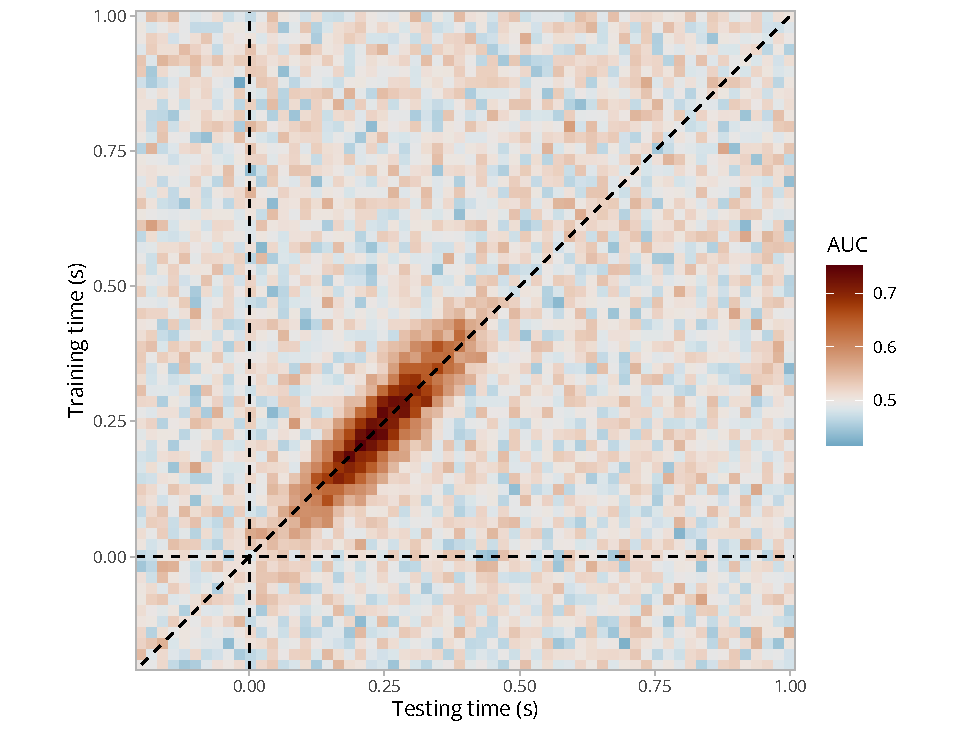
\includegraphics[width=1\textwidth,height=\textheight]{brms_meeg_files/figure-pdf/fig-sim-timegen-1.pdf}

}

\end{figure}%

Now, we want to test whether and when decoding performance is above
chance level (0.5 for a binary decoding task). These two models are
computationally heavier to fit (more observations and 2D smooth
functions)\ldots{}

\begin{Shaded}
\begin{Highlighting}[]
\CommentTok{\# fitting a GAM with two temporal dimensions}
\NormalTok{timegen\_gam }\OtherTok{\textless{}{-}} \FunctionTok{brm}\NormalTok{(}
    \CommentTok{\# 2D thin{-}plate spline (tp)}
\NormalTok{    auc }\SpecialCharTok{\textasciitilde{}} \FunctionTok{t2}\NormalTok{(train\_time, test\_time, }\AttributeTok{bs =} \StringTok{"tp"}\NormalTok{, }\AttributeTok{k =} \DecValTok{20}\NormalTok{),}
    \AttributeTok{data =}\NormalTok{ timegen\_data,}
    \AttributeTok{family =} \FunctionTok{Beta}\NormalTok{(),}
    \AttributeTok{iter =} \DecValTok{5000}\NormalTok{,}
    \AttributeTok{chains =} \DecValTok{4}\NormalTok{,}
    \AttributeTok{cores =} \DecValTok{4}\NormalTok{,}
    \AttributeTok{file =} \StringTok{"models/timegen\_gam\_t2.rds"}
\NormalTok{    )}

\CommentTok{\# fitting a GP with two temporal dimensions}
\CommentTok{\# timegen\_gp \textless{}{-} brm(}
\CommentTok{\#     auc \textasciitilde{} gp(train\_time, test\_time, k = 20),}
\CommentTok{\#     data = timegen\_data,}
\CommentTok{\#     family = Beta(),}
\CommentTok{\#     control = list(adapt\_delta = 0.95),}
\CommentTok{\#     iter = 2000,}
\CommentTok{\#     chains = 4,}
\CommentTok{\#     cores = 4,}
\CommentTok{\#     file = "models/timegen\_gp.rds"}
\CommentTok{\#     )}
\end{Highlighting}
\end{Shaded}

\begin{figure}[H]

\caption{Posterior probability of decoding accuracy being above chance
level (2D GAM).}

{\centering 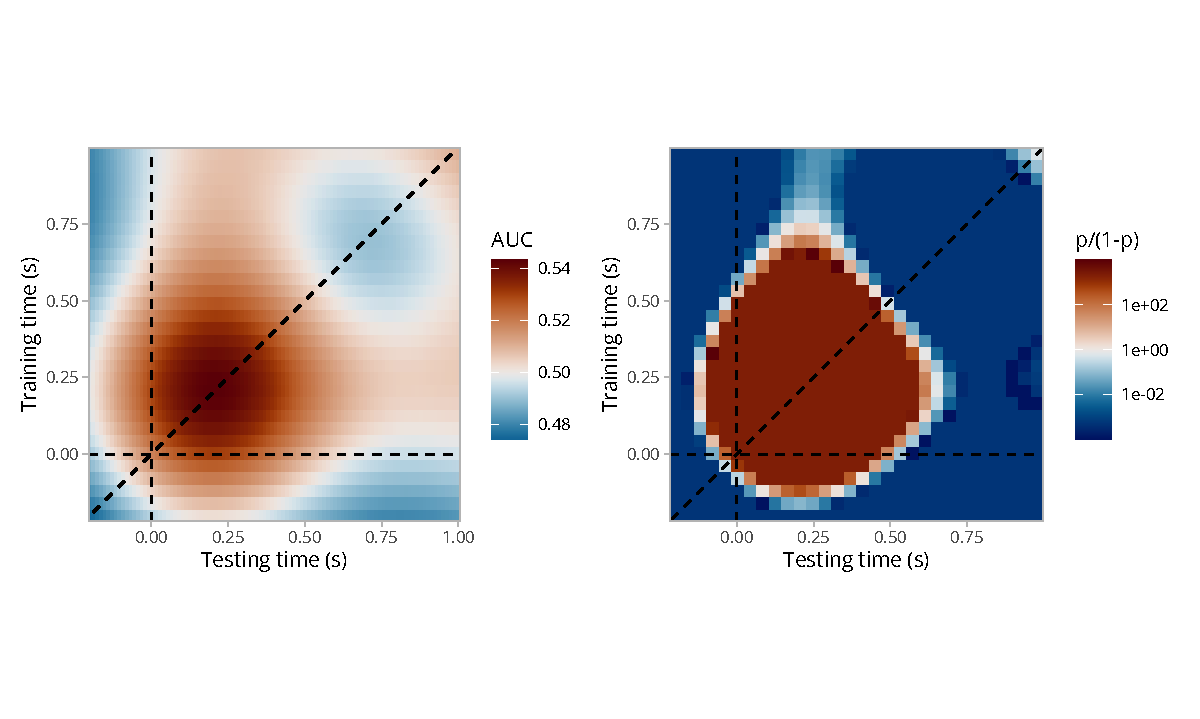
\includegraphics[width=1\textwidth,height=\textheight]{brms_meeg_files/figure-pdf/gam-timegen-post-preds-1.pdf}

}

\end{figure}%

Could be extended to spatial and temporal dimensions with formulas such
as \texttt{te(x,\ y,\ Time,\ d\ =\ c(2,\ 1)\ )}\ldots{}

\newpage

\section{Mathematical formulation of the bivariate
GAM}\label{mathematical-formulation-of-the-bivariate-gam}

To model cross-temporal generalisation matrices of decoding performance
(ROC AUC), we extended the initial (decoding) GAM to take into account
the bivariate temporal distribution of AUC values, thus producing
naturally smoothed estimates (timecourses) of AUC values and posterior
probabilities. This model can be written as follows:

\[
\begin{aligned}
\text{AUC}_{i} &\sim \mathrm{Beta}(\mu_{i}, \phi)\\
g(\mu_{i}) &= f \left(\text{train}_{i}, \text{test}_{i} \right)\\
\end{aligned}
\]

where we assume that AUC values come from a \(\mathrm{Beta}\)
distribution with two parameters \(\mu\) and \(\phi\). We can think of
\(f \left(\text{train}_{i}, \text{test}_{i} \right)\) as a surface (a
smooth function of two variables) that we can model using a
2-dimensional splines. Let
\(\mathbf{s}_{i} = \left(\text{train}_{i}, \text{test}_{i} \right)\) be
some pair of training and testing samples, and let
\(\mathbf{k}_{m} = \left(\text{train}_{m}, \text{test}_{m} \right)\)
denote the \(m^{\text{th}}\) knot in the domain of \(\text{train}_{i}\)
and \(\text{test}_{i}\). We can then express the smooth function as:

\[
f \left(\text{train}_{i}, \text{test}_{i} \right) = \alpha + \sum_{m=1}^M \beta_{m} b_{m} \left(\tilde{s}_{i}, \tilde{k}_{m} \right)
\]

Note that \(b_{m}(,)\) is a basis function that maps
\(R \times R \rightarrow R\). A popular bivariate basis function uses
\emph{thin-plate splines} (\citeproc{ref-wood2003}{Wood, 2003}), which
extend to \(\mathbf{s}_{i} \in \mathbb{R}^{d}\) and \(\partial l_{g}\)
penalties. These splines are designed to interpolate and approximate
smooth surfaces over two dimensions (hence the ``bivariate'' term). For
\(d=2\) dimensions and \(l=2\) (smoothness penalty involving second
order derivative):

\[
f \left(\tilde{s}_{i} \right) = \alpha + \beta_{1} x_{i} + \beta_{2} z_{i} +\sum_{m=1}^{M} \beta_{2+m} b_m\left(\tilde{s}_i, \tilde{k}_m\right)
\]

using the the radial basis function given by:

\[
b_m\left(\tilde{s}_i, \tilde{k}_m\right)=\left\|\tilde{s}_i-\tilde{k}_m\right\|^2 \log \left\|\tilde{s}_i-\tilde{k}_m\right\|
\]

where \(\left\|\mathbf{s}_i-\mathbf{k}_{m}\right\|\) is the Euclidean
distance between the covariate \(\mathbf{s}_{i}\) and the knot location
\(\mathbf{k}_{m}\).

\newpage

\section{\texorpdfstring{Integration with
\texttt{MNE-Python}}{Integration with MNE-Python}}\label{integration-with-mne-python}

Explain how to use the \texttt{R} package with \texttt{MNE}
epochs\ldots{}

\begin{Shaded}
\begin{Highlighting}[]
\CommentTok{\# TO{-}DO: adding some code here...}
\end{Highlighting}
\end{Shaded}







\end{document}
